\documentclass[xcolor={dvipsnames},aspectratio=169,10pt]{beamer}
% utility packages
\usepackage{etoolbox}
\usepackage{multicol}
\usepackage{relsize}
\usepackage{fontawesome}

% better text justifying
\usepackage{microtype}
% justify text inside list environment
% Ref: http://liam0205.me/2017/04/11/justifying-in-beamer-s-lists/
\usepackage{ragged2e}
\makeatletter
\patchcmd{\itemize}{\raggedright}{\justifying}{}{}
\patchcmd{\beamer@enum@}{\raggedright}{\justifying}{}{}
\patchcmd{\@@description}{\raggedright}{\justifying}{}{}
\makeatother

% table of content with numbers and justification
% https://tex.stackexchange.com/questions/188773
\setbeamertemplate{section in toc}{\hspace*{1em}\inserttocsectionnumber.~\inserttocsection\par}
\setbeamertemplate{subsection in toc}{\hspace*{2em}\inserttocsectionnumber.\inserttocsubsectionnumber.~\inserttocsubsection\par}

% math related packages
\usepackage{amsmath}
\usepackage[ruled,vlined]{algorithm2e}
\SetAlCapNameFnt{\scriptsize}
\SetAlCapFnt{\scriptsize}
\SetAlFnt{\scriptsize}

% figure related packages
\usepackage{graphicx}
\usepackage[scale=2]{ccicons}
\usepackage{qrcode}
\usepackage{tikz}
\usepackage{tikzpagenodes}
\usetikzlibrary{positioning}

% table related packages
\usepackage{array}
\usepackage{booktabs}
\usepackage{multirow}
\usepackage{colortbl}
\newcommand{\tabincell}[2]{\begin{tabular}{@{}#1@{}}#2\end{tabular}}

% code highlight
\usepackage{listings}
\usepackage{minted}
\definecolor{mintedbg}{HTML}{E5E9F0}
\setminted{autogobble,bgcolor=mintedbg,fontsize=\small}
\setmintedinline{bgcolor=mintedbg,fontsize=\smaller}
\newminted{bash}{}
\newminted{latex}{}
\newmintinline{bash}{}
\newmintinline{latex}{}
\newcommand{\texdoc}[2]{\href{#2}{\bashinline|texdoc #1|}}

% hyperref setting
\hypersetup{
  unicode,
  psdextra,
  bookmarksnumbered=true,
  bookmarksopen=true,
  bookmarksopenlevel=3,
  bookmarksdepth=4,
  pdfcenterwindow=true,
  pdfstartview={Fit},
  pdfpagemode={FullScreen},
  pdfpagelayout={SinglePage},
}
\usepackage{bookmark}

% beamer theme
\usetheme{metropolis}
\metroset{block=fill,numbering=fraction}

% caption style
\usepackage{subcaption}
\setlength\abovecaptionskip{3pt}
\setbeamerfont{caption}{size=\scriptsize}
\renewcommand{\figurename}{Fig.}
\captionsetup{labelformat=empty,labelsep=none,textfont={bf,it}}

% Ref: https://github.com/gpoore/minted/blob/master/source/minted.dtx
\newenvironment{latexexample}
{\VerbatimEnvironment\begin{VerbatimOut}[gobble=3]{example.out}}{\end{VerbatimOut}%
  \begin{center}
    \begin{minipage}{0.47\linewidth}%
      \inputminted[resetmargins,fontsize=\scriptsize]{latex}{example.out}%
    \end{minipage}%
    \hspace{0.05\linewidth}%
    \begin{minipage}{0.47\linewidth}%
      \begin{framed}
        \setlength{\parindent}{2em}%
        \input{example.out}%
      \end{framed}
    \end{minipage}%
  \end{center}
}

\newenvironment{mathexample}
{\VerbatimEnvironment\begin{VerbatimOut}[gobble=3]{example.out}}{\end{VerbatimOut}%
  \begin{center}
    \begin{minipage}{0.47\linewidth}%
      \inputminted[resetmargins,fontsize=\scriptsize]{latex}{example.out}%
    \end{minipage}%
    \hspace{0.05\linewidth}%
    \begin{minipage}{0.47\linewidth}%
      \begin{framed}
        \[ \input{example.out} \]
      \end{framed}
    \end{minipage}%
  \end{center}
}

\newenvironment{mathexamples}
{\VerbatimEnvironment\begin{VerbatimOut}[gobble=3]{example.out}}{\end{VerbatimOut}%
  \begin{center}
    \begin{minipage}{0.47\linewidth}%
      \inputminted[resetmargins,fontsize=\scriptsize]{latex}{example.out}%
    \end{minipage}%
    \hspace{0.05\linewidth}%
    \begin{minipage}{0.47\linewidth}%
      \begin{framed}
        \directlua{
          local first = true
          for line in io.lines('example.out') do
          if first then
          first = false
          else
          tex.print('\\newline ')
          end
          tex.print('$' .. line .. '$')
          end
        }
      \end{framed}
    \end{minipage}%
  \end{center}
}


%-----------------------------------------------------------
% Add Paper using {\paper{}. begin{beawer} ... end{beamer} }
%-----------------------------------------------------------
\newcommand\paper[1]{
	\setbeamertemplate{footline}
	{
		\begin{beamercolorbox}[wd=\textwidth,ht=3mm,dp=03mm,leftskip=0.3cm,rightskip=0.3cm]{black}%
        		\usebeamerfont{page number in head/foot}
			(#1)\mbox{}\hfill\insertframenumber/\inserttotalframenumber 
		\end{beamercolorbox}%
	}
}



\title{Nonlinear analysis to quantify human movement variability from time-series data}
\subtitle{Seminario Virtual \faTwitter @todoscicese \#svcicese}
\author{ \textbf{Miguel Xochicale, PhD} [\faTwitter @\_mxochicale \faGithub @mxochicale]
}

\institute{
	School of Biomedical Engineering and Imaging Sciences \\
	King's College London
	}

\date{November 27, 2020; 12h00m GMT-8
	%Seminario Virtual \faTwitter @todoscicese \#svcicese
}



\titlegraphic{
  \begin{tikzpicture}[overlay, remember picture]
    \node[%
      above right=0.35cm and -0.2cm of current page footer area.south west,
      anchor=south west,
      inner sep=0pt] {%
      \usebeamerfont{footline}
      \begin{tabular}{lm{.8\textwidth}}
        \href{http://creativecommons.org/licenses/by/4.0/}{\ccby} &
        This work is licensed under a \href{http://creativecommons.org/licenses/by/4.0/}{Creative Commons ``Attribution 4.0 International''} license. \par
        Get source of this slides and example document from \url{https://github.com/mxochicale/seminario-cicese-27112020}.
      \end{tabular}
    };
    \node[%
      above left=0.35cm and 0cm of current page footer area.south east,
      anchor=south east,
      inner sep=0pt]{\qrcode[height=1.5cm]{https://github.com/mxochicale/seminario-cicese-27112020}};
  \end{tikzpicture}
}

\begin{document}
\maketitle

%\begin{frame}{Contents}
%  \setbeamertemplate{section in toc}[sections numbered]
%  \tableofcontents[hideallsubsections]
%\end{frame}

\begin{frame}{Contents}
    \tableofcontents
\end{frame}



%%%%% CONTENT %%%%%%%
%%%%%%%%%%%%%%%%%%%%%%%%%%%%%%%%%%%%%%%%%%%%
\section{Short-bio}


\begin{frame}{My journey in science}

\begin{itemize}	
	\item \textbf{(1996-1999)} High School in Electronics
	\item \textbf{(1999-2004)} BSc in Electronics  
	\item \textbf{(2004-2006)} MSc in Signal Processing 
	\item \textbf{(2006-2012)} Teaching Associate in Mechatronics 
	\item \textbf{(2013-2014)} Research Assistant in Robotics at INAOE  
	\item \textbf{(2014-2019)} PhD student in Human-Robot Interaction at Uni of Bham \\
	\item \textbf{(2019-present)} Research Associate in Ultrasound-Guidance 
	Intervention at KCL 
\end{itemize}

	\vspace{4mm}
        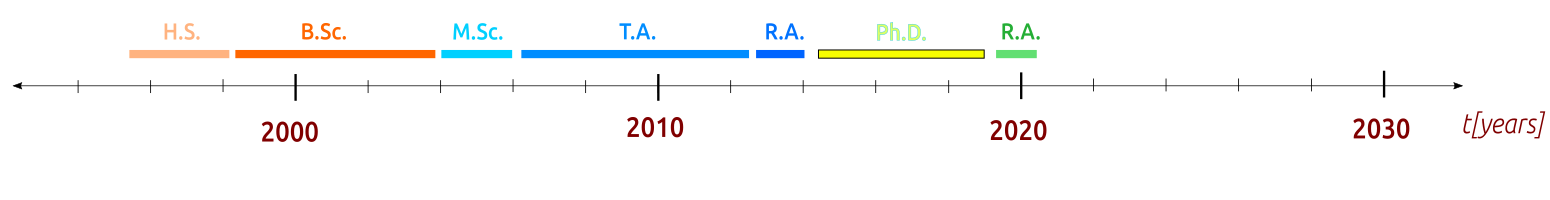
\includegraphics[width=\linewidth]{./figs/myjourney/versions/drawing.png}

\end{frame}






%%%%%%%%%%%%%%%%%%%%%%%%%%%%%%%%%%%%%%%%%%%%
\section{Nonlinear analysis to quantify human movement variability from time-series data}
\subsection{Why Movement Variability?}


{
%\paper{
%Bernstein 1967 in \textbf{The co-ordination and regulation of movements};
%}
\begin{frame}[fragile]{Few challenges when quantifying movement variability}
  \begin{columns}
   

 \begin{column}{.3\linewidth}
    
	\textbf{Theoretical challenges}
  \begin{itemize}
        \item Modelling human movement (tasks, environments, agent, perception, action)
        \item Modelling human variability (complexity vs predictability)
        \item ?
      \end{itemize}
    \end{column}

   \begin{column}{.3\linewidth}
	
	\textbf{Choosing the right tools} 
           \begin{itemize}
                \item Time-based domain,
		\item Frequency-based domain
		\item Nonlinear dynamics
                \item ?
              \end{itemize}
	\end{column}

   \begin{column}{.3\linewidth}
	\textbf{Technical challenges}
           \begin{itemize}
                \item non-stationarity, 
		\item non-linearity, 
		\item data length, 
		\item sensor source, 
		\item noise,
                \item ?
              \end{itemize}
	\end{column}



  \end{columns}


\end{frame}
}



%%%%%%%%%%%%%%%%%%%%%%%%%%%%%%%%%%%%%%%%%%%%%%%%%%%%%%%%
{
\paper{
Bernstein 1967 in \textbf{The co-ordination and regulation of movements};
Newell and Vaillancourt 2001 in \textbf{Hum Mov Sci};
Davids et al. 2003 in \textbf{Sport Medicine};
Warren 2006 in \textbf{Psychological Review}
}
\begin{frame}{Modeling Human Movement}
    \begin{figure}
        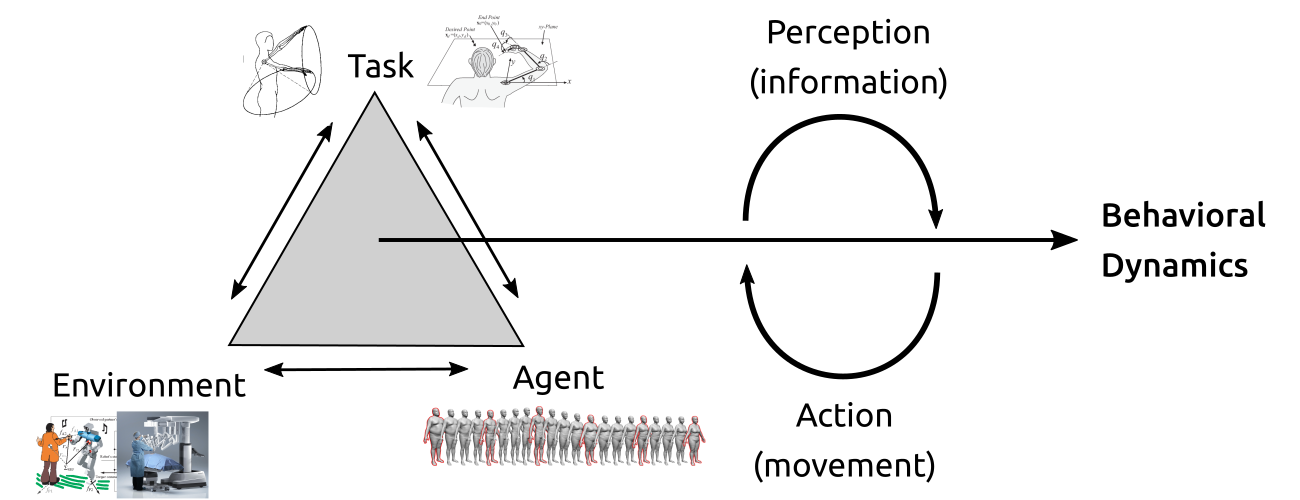
\includegraphics[width=1.0\linewidth]{./figs/modeling-movement/versions/drawing-v01.png}
	%\caption{Newell's model of movement constrains} 
   \end{figure}
\end{frame}
}



%%%%%%%%%%%%%%%%%%%%%%%%%%%%%%%%%%%%%%%%%%%%%%%%%%%%%%%%
{
\paper{
Stergiou et al. 2006 in {\bf Neurologic Physical Therapy};
Stergiou and Decker 2011 in {\bf Human Movement Science};
Tononi et al. 1998 in {\bf Trends in Cognitive Sciences}
}
\begin{frame}{Modelling Movement Variability}
    \begin{figure}
        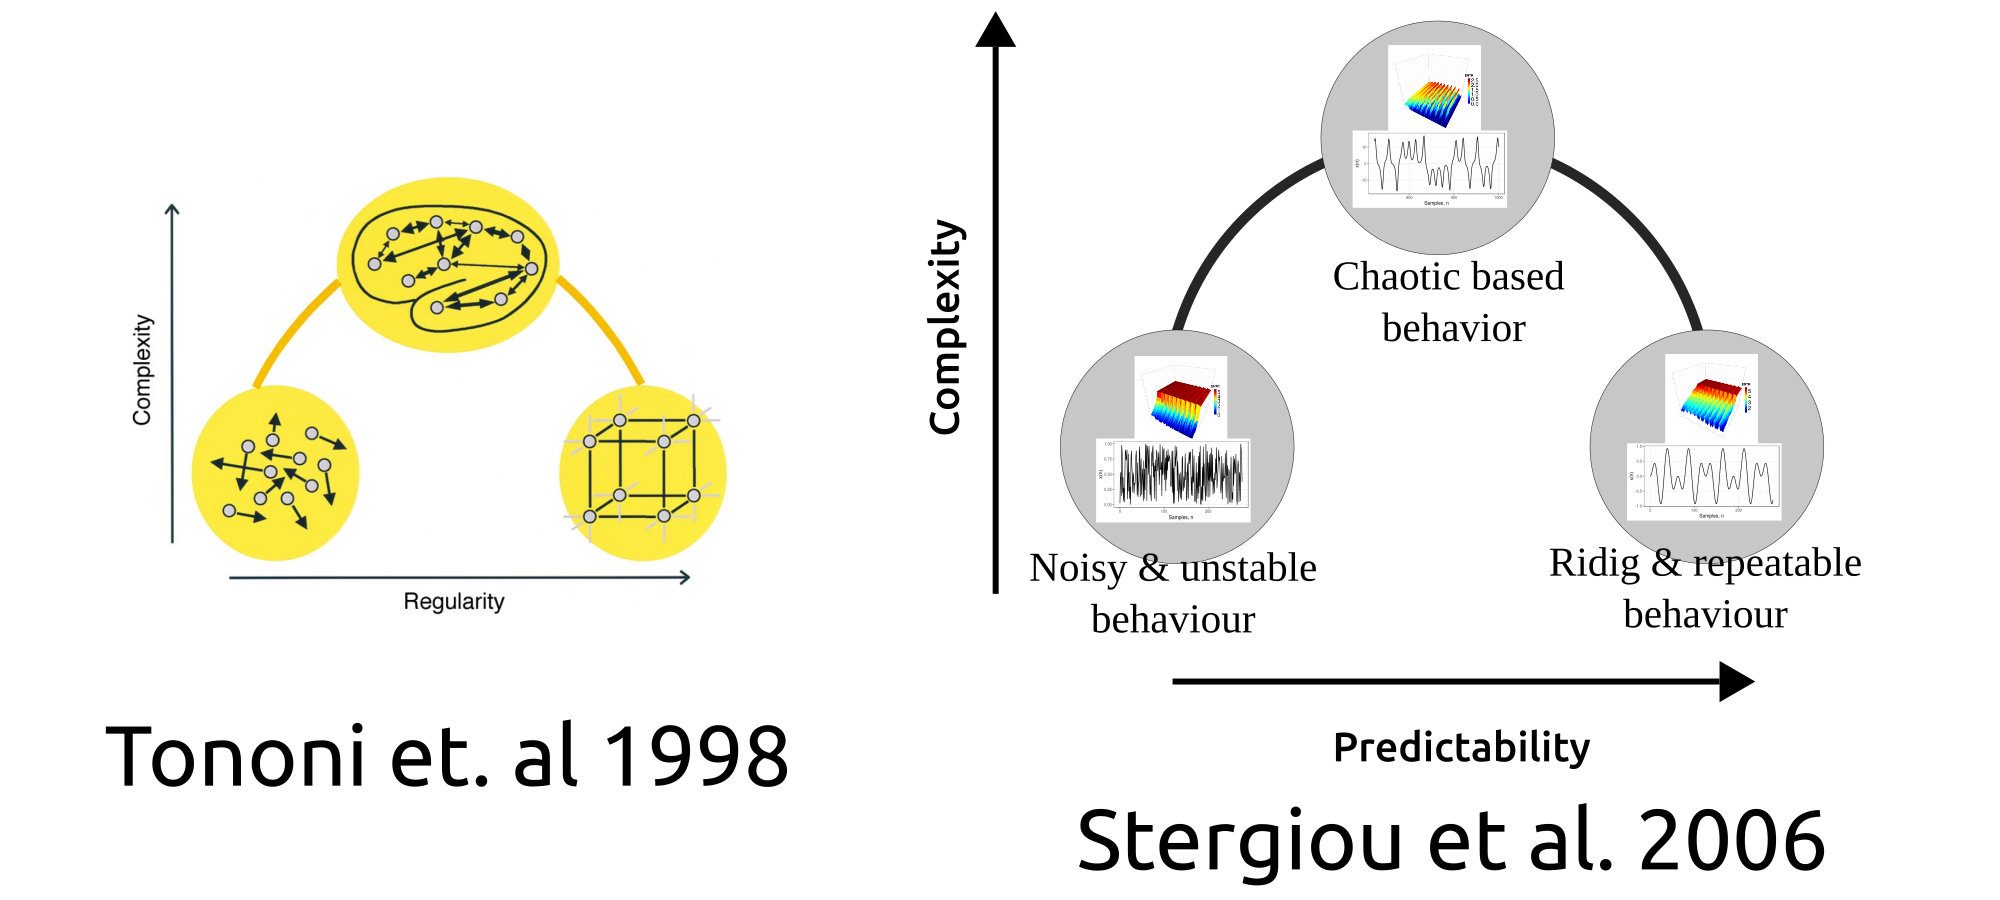
\includegraphics[width=0.95\linewidth]{./figs/modeling-movement-variability/versions/drawing-v00.png}
	%\caption{Theoretical Model of Optimal Movement Variability}
   \end{figure}
\end{frame}
}


%%%%%%%%%%%%%%%%%%%%%%%%%%%%%%%%%%%%%%%%%%%%
\subsection{Nonlinear Methods}

{
\paper{
M. Xochicale 2019 in \textbf{PhD thesis} 
}
\begin{frame}{Nonlinear Analysis}
    \vspace{-00mm}
      \begin{figure}
        \centering
        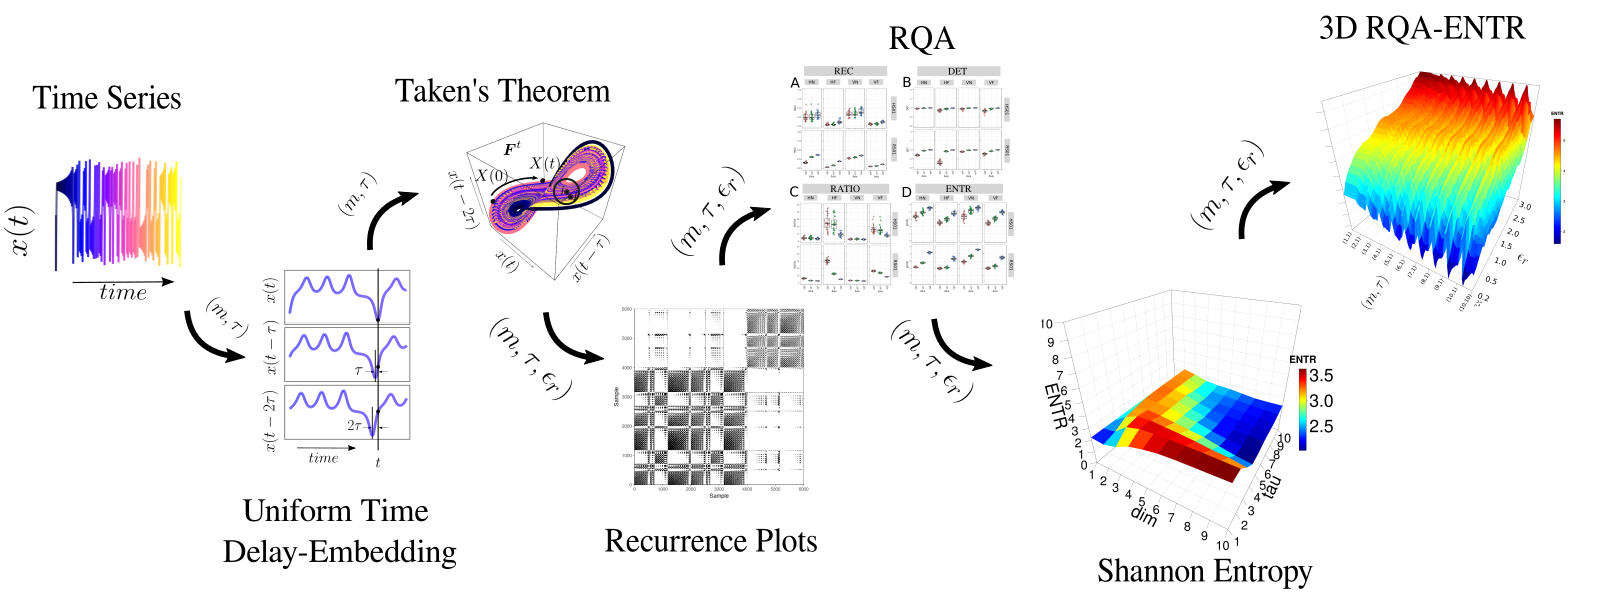
\includegraphics[width=0.99\linewidth]{./figs/nonlinear-methods/versions/drawing-v00.png}
        \caption{}
      \end{figure}
\end{frame}
}

\subsection{Experiment/Results}

{
\paper{Xochicale 2019 in {\bf PhD thesis} }
\begin{frame}{Human-Humanoid Imitation Activities}
20 participants with mean and standard deviation (SD) age of 
mean=19.8 (SD=1.39) years, being four females and sixteen males.
    \begin{figure}
        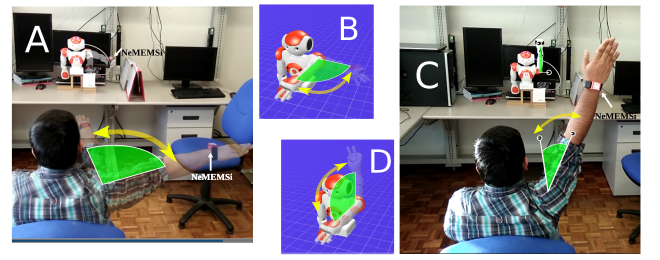
\includegraphics[width=0.9\linewidth]{./figs/experiment/versions/drawing-v00}{}
	\caption[PA]{(A/C) Front-to-Front Human-Humanoid Imitation 
		Activities of Horizontal/Vertical Movements,
		(B/D) NAO, humanoid robot, performing 
		Horizontal/Vertical arm movements.
		}
   \end{figure}
\end{frame}
}




%%%%%%%%%%%%%%%%%%%%%%%%%%%%%%%%%%%%%%%%%%%%%%%%%%%%%%%%%%
{
\paper{Xochicale 2019 in {\bf PhD Thesis}}
\begin{frame}{From Raw to Smoothed Time Series}
   \begin{figure}
        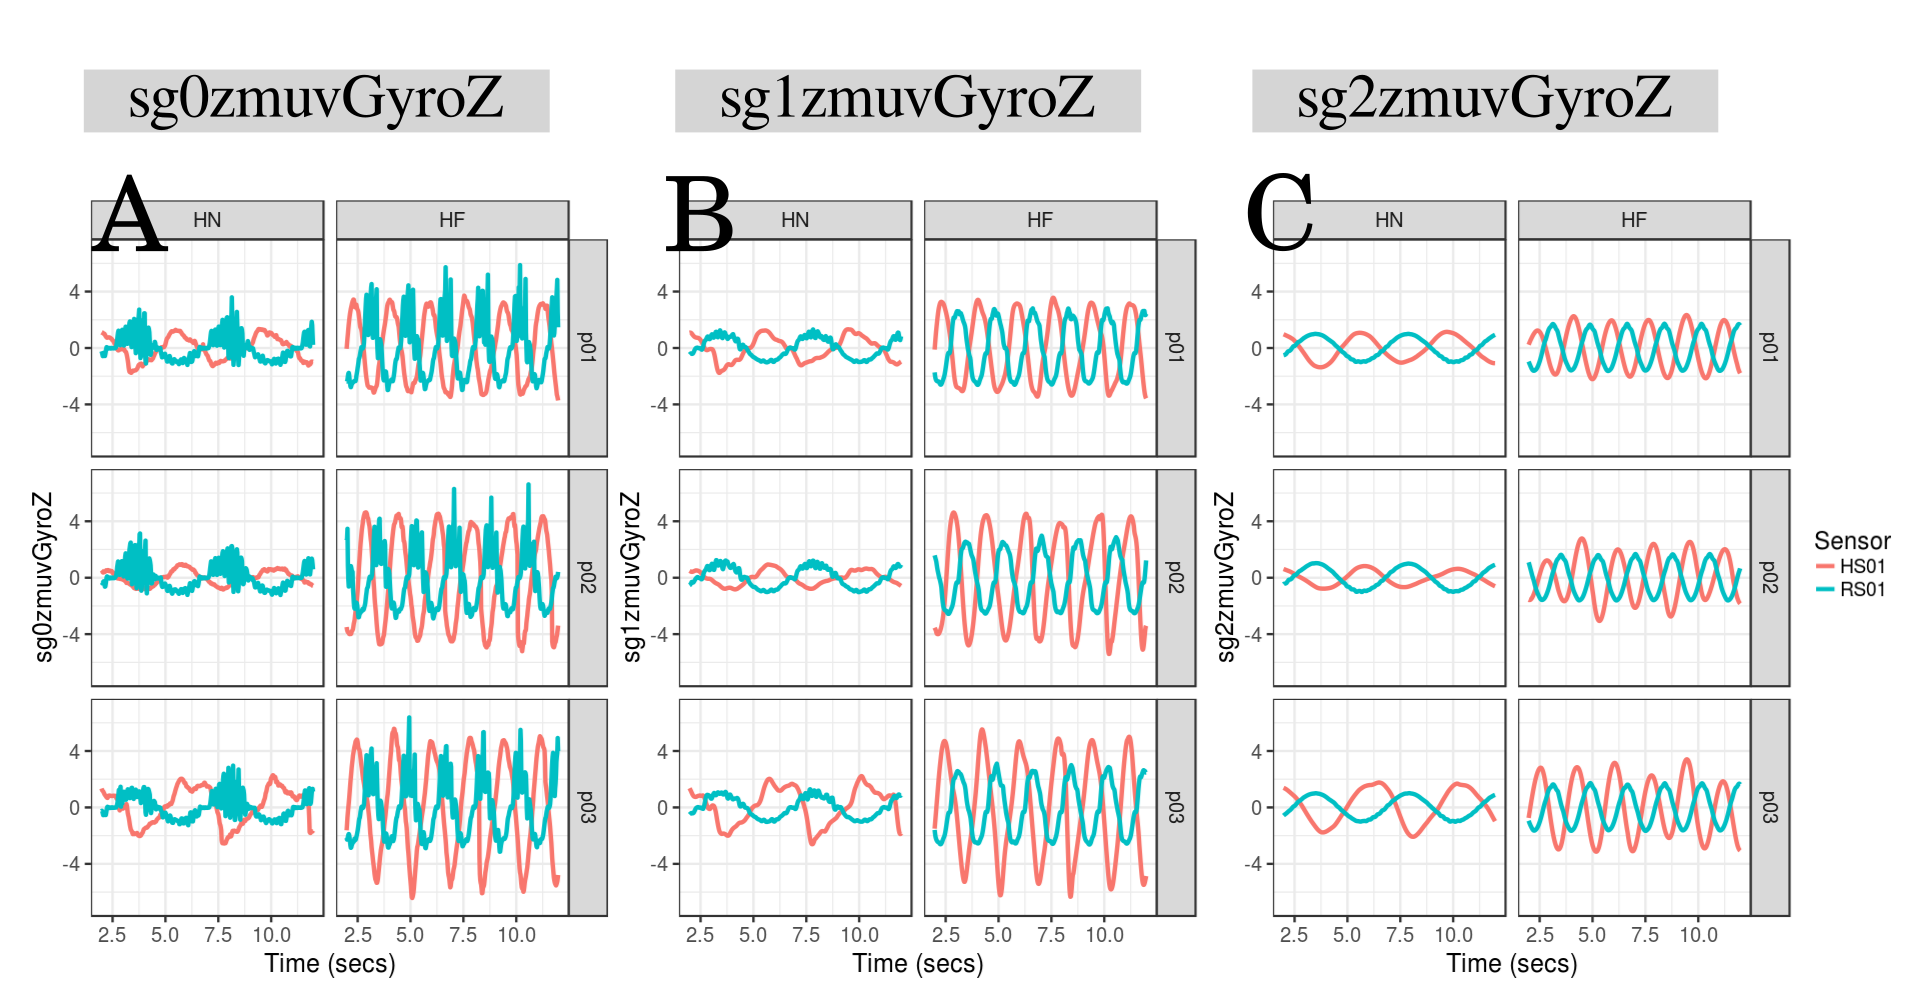
\includegraphics[width=0.9\linewidth]{./figs/results/ch6-ts-h/versions/drawing-v00}{}
	\caption{Time-series of horizontal movements for 
	(A) normalised, (B) \texttt{sgolay(p=5,n=25)}, and 
	(C) \texttt{sgolay(p=5,n=159).} } 
   \end{figure}
\end{frame}
}


%%%%%%%%%%%%%%%%%%%%%%%%%%%%%%%%%%%%%%%%%%%%%%%%%%%%%%%%%%
{
\paper{Xochicale 2019 in {\bf PhD Thesis}}
\begin{frame}{From Raw to Smoothed Time Series}
   \begin{figure}
        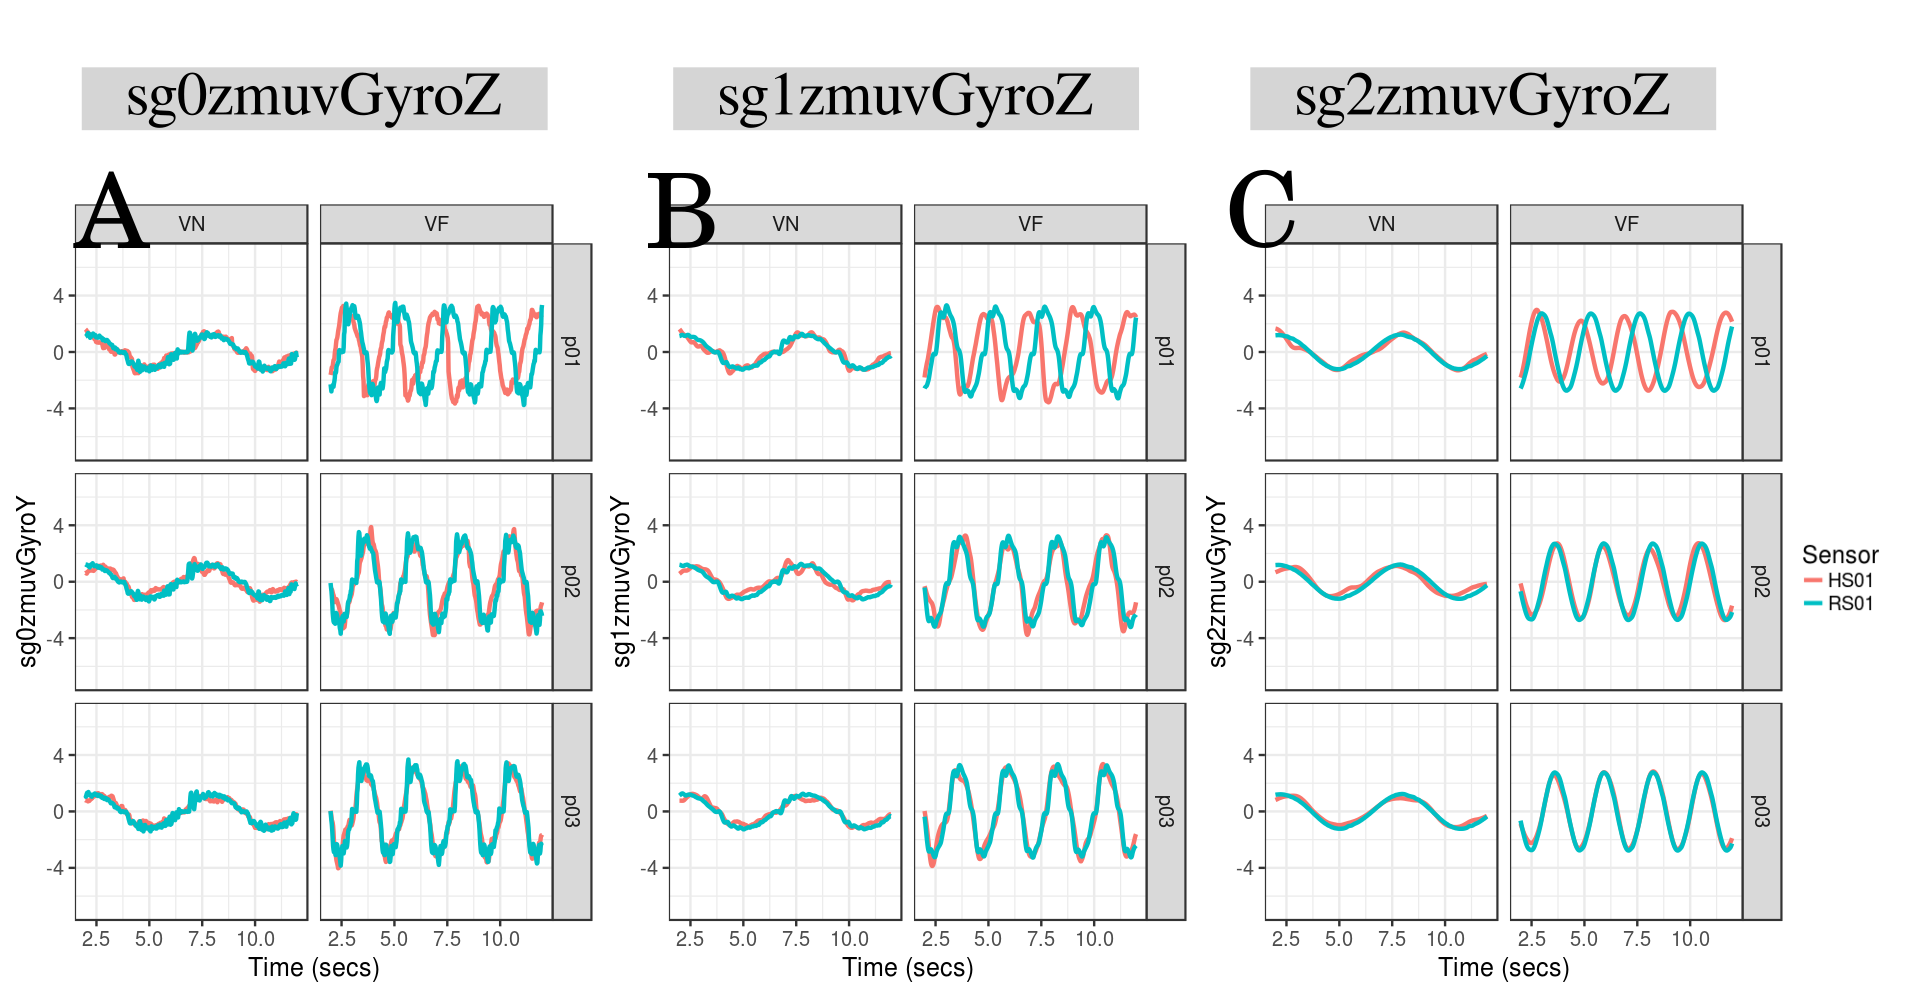
\includegraphics[width=0.9\linewidth]{./figs/results/ch6-ts-v/versions/drawing-v00}{}
	\caption{Time-series of vertical movements for 
	(A) normalised, (B) \texttt{sgolay(p=5,n=25)}, and 
	(C) \texttt{sgolay(p=5,n=159).} } 
   \end{figure}
\end{frame}
}



%%%%%%%%%%%%%%%%%%%%%%%%%%%%%%%%%%%%%%%%%%%%%%%%%%%%%%%%%
{
\paper{Xochicale 2019 in {\bf PhD Thesis}}
\begin{frame}{Minimum Embedding Parameters}
    \begin{figure}
        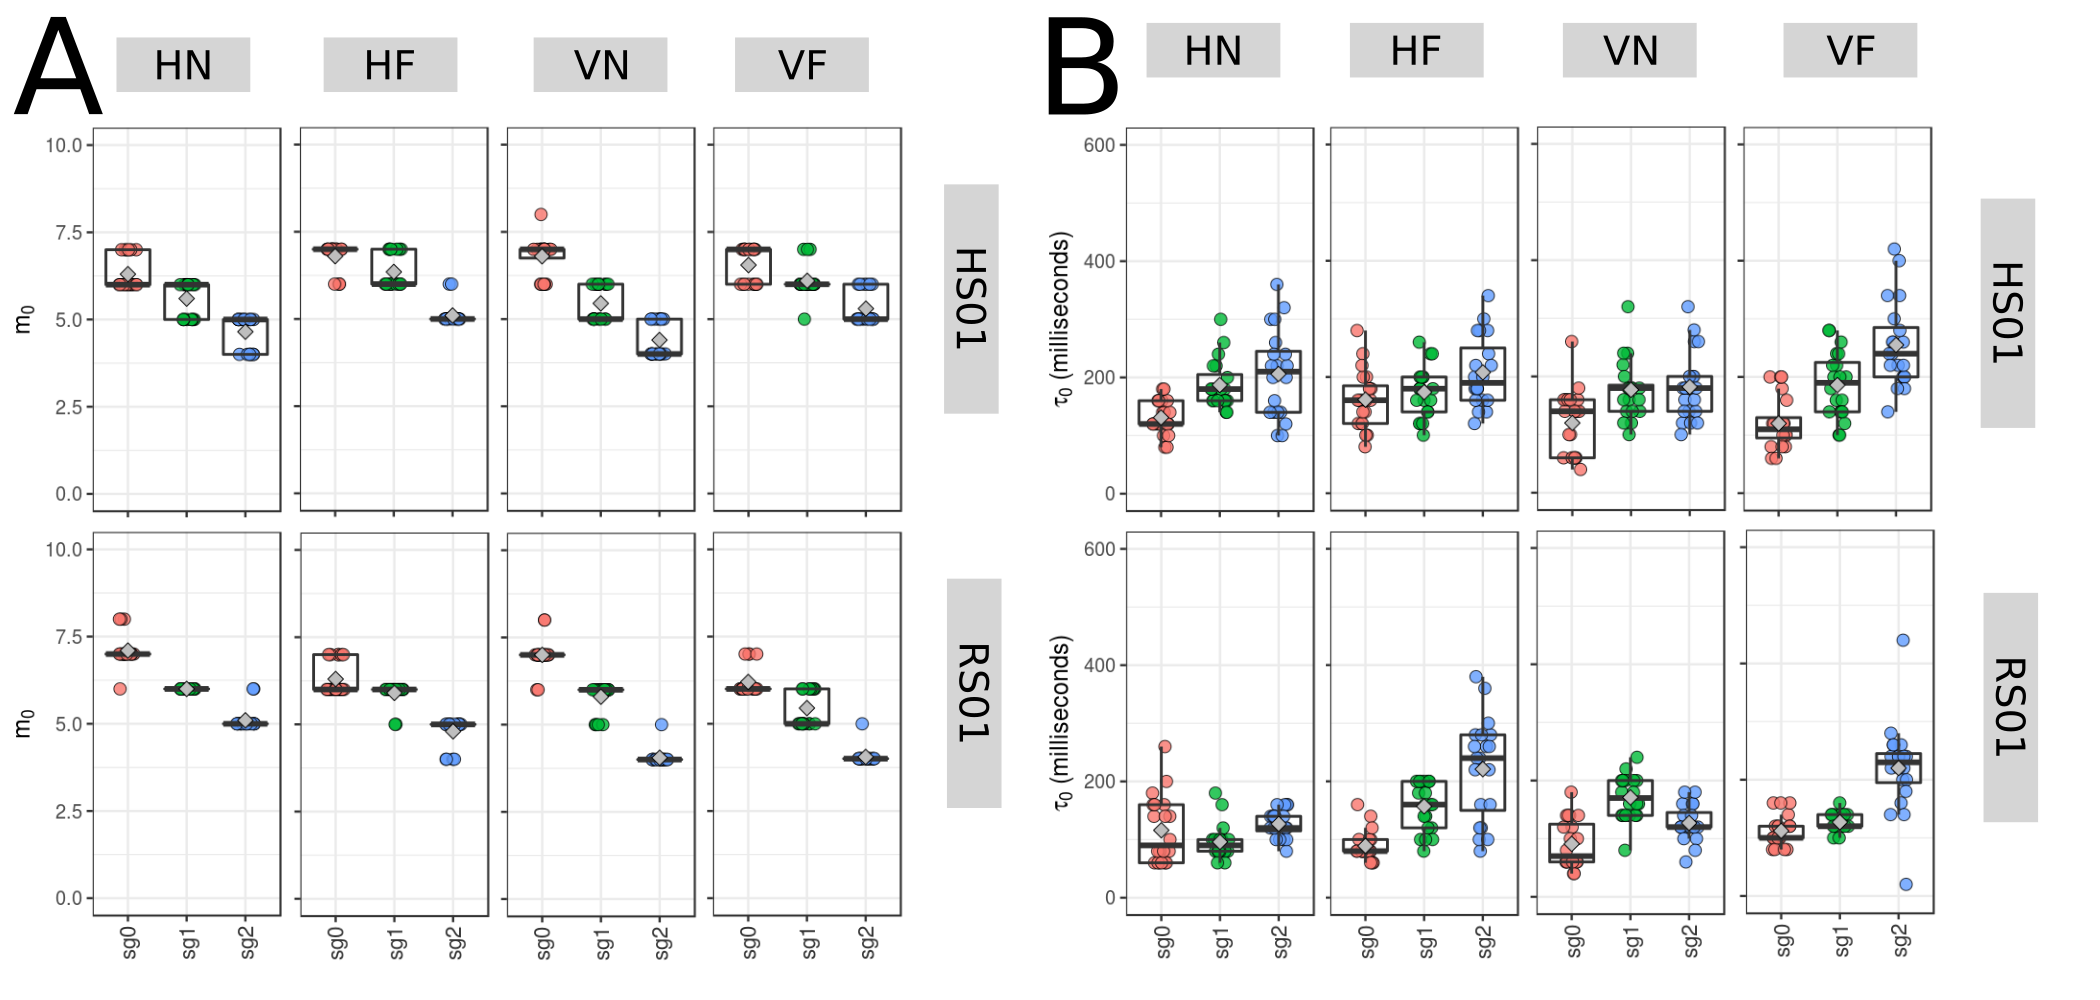
\includegraphics[width=0.9\linewidth]{./figs/results/ch6-empa/versions/drawing-v00}{}
	\caption{(A) Minimum Embedding Dimension 
		 (B) First Minimum AMI
		}  
   \end{figure}
	
\end{frame}
}


%%%%%%%%%%%%%%%%%%%%%%%%%%%%%%%%%%%%%%%%%%%%%%%%%%%%%%%%
{
%\paper{Xochicale 2019 in {\bf PhD Thesis}}
\begin{frame}{Reconstructed State Spaces}
    \begin{figure}
        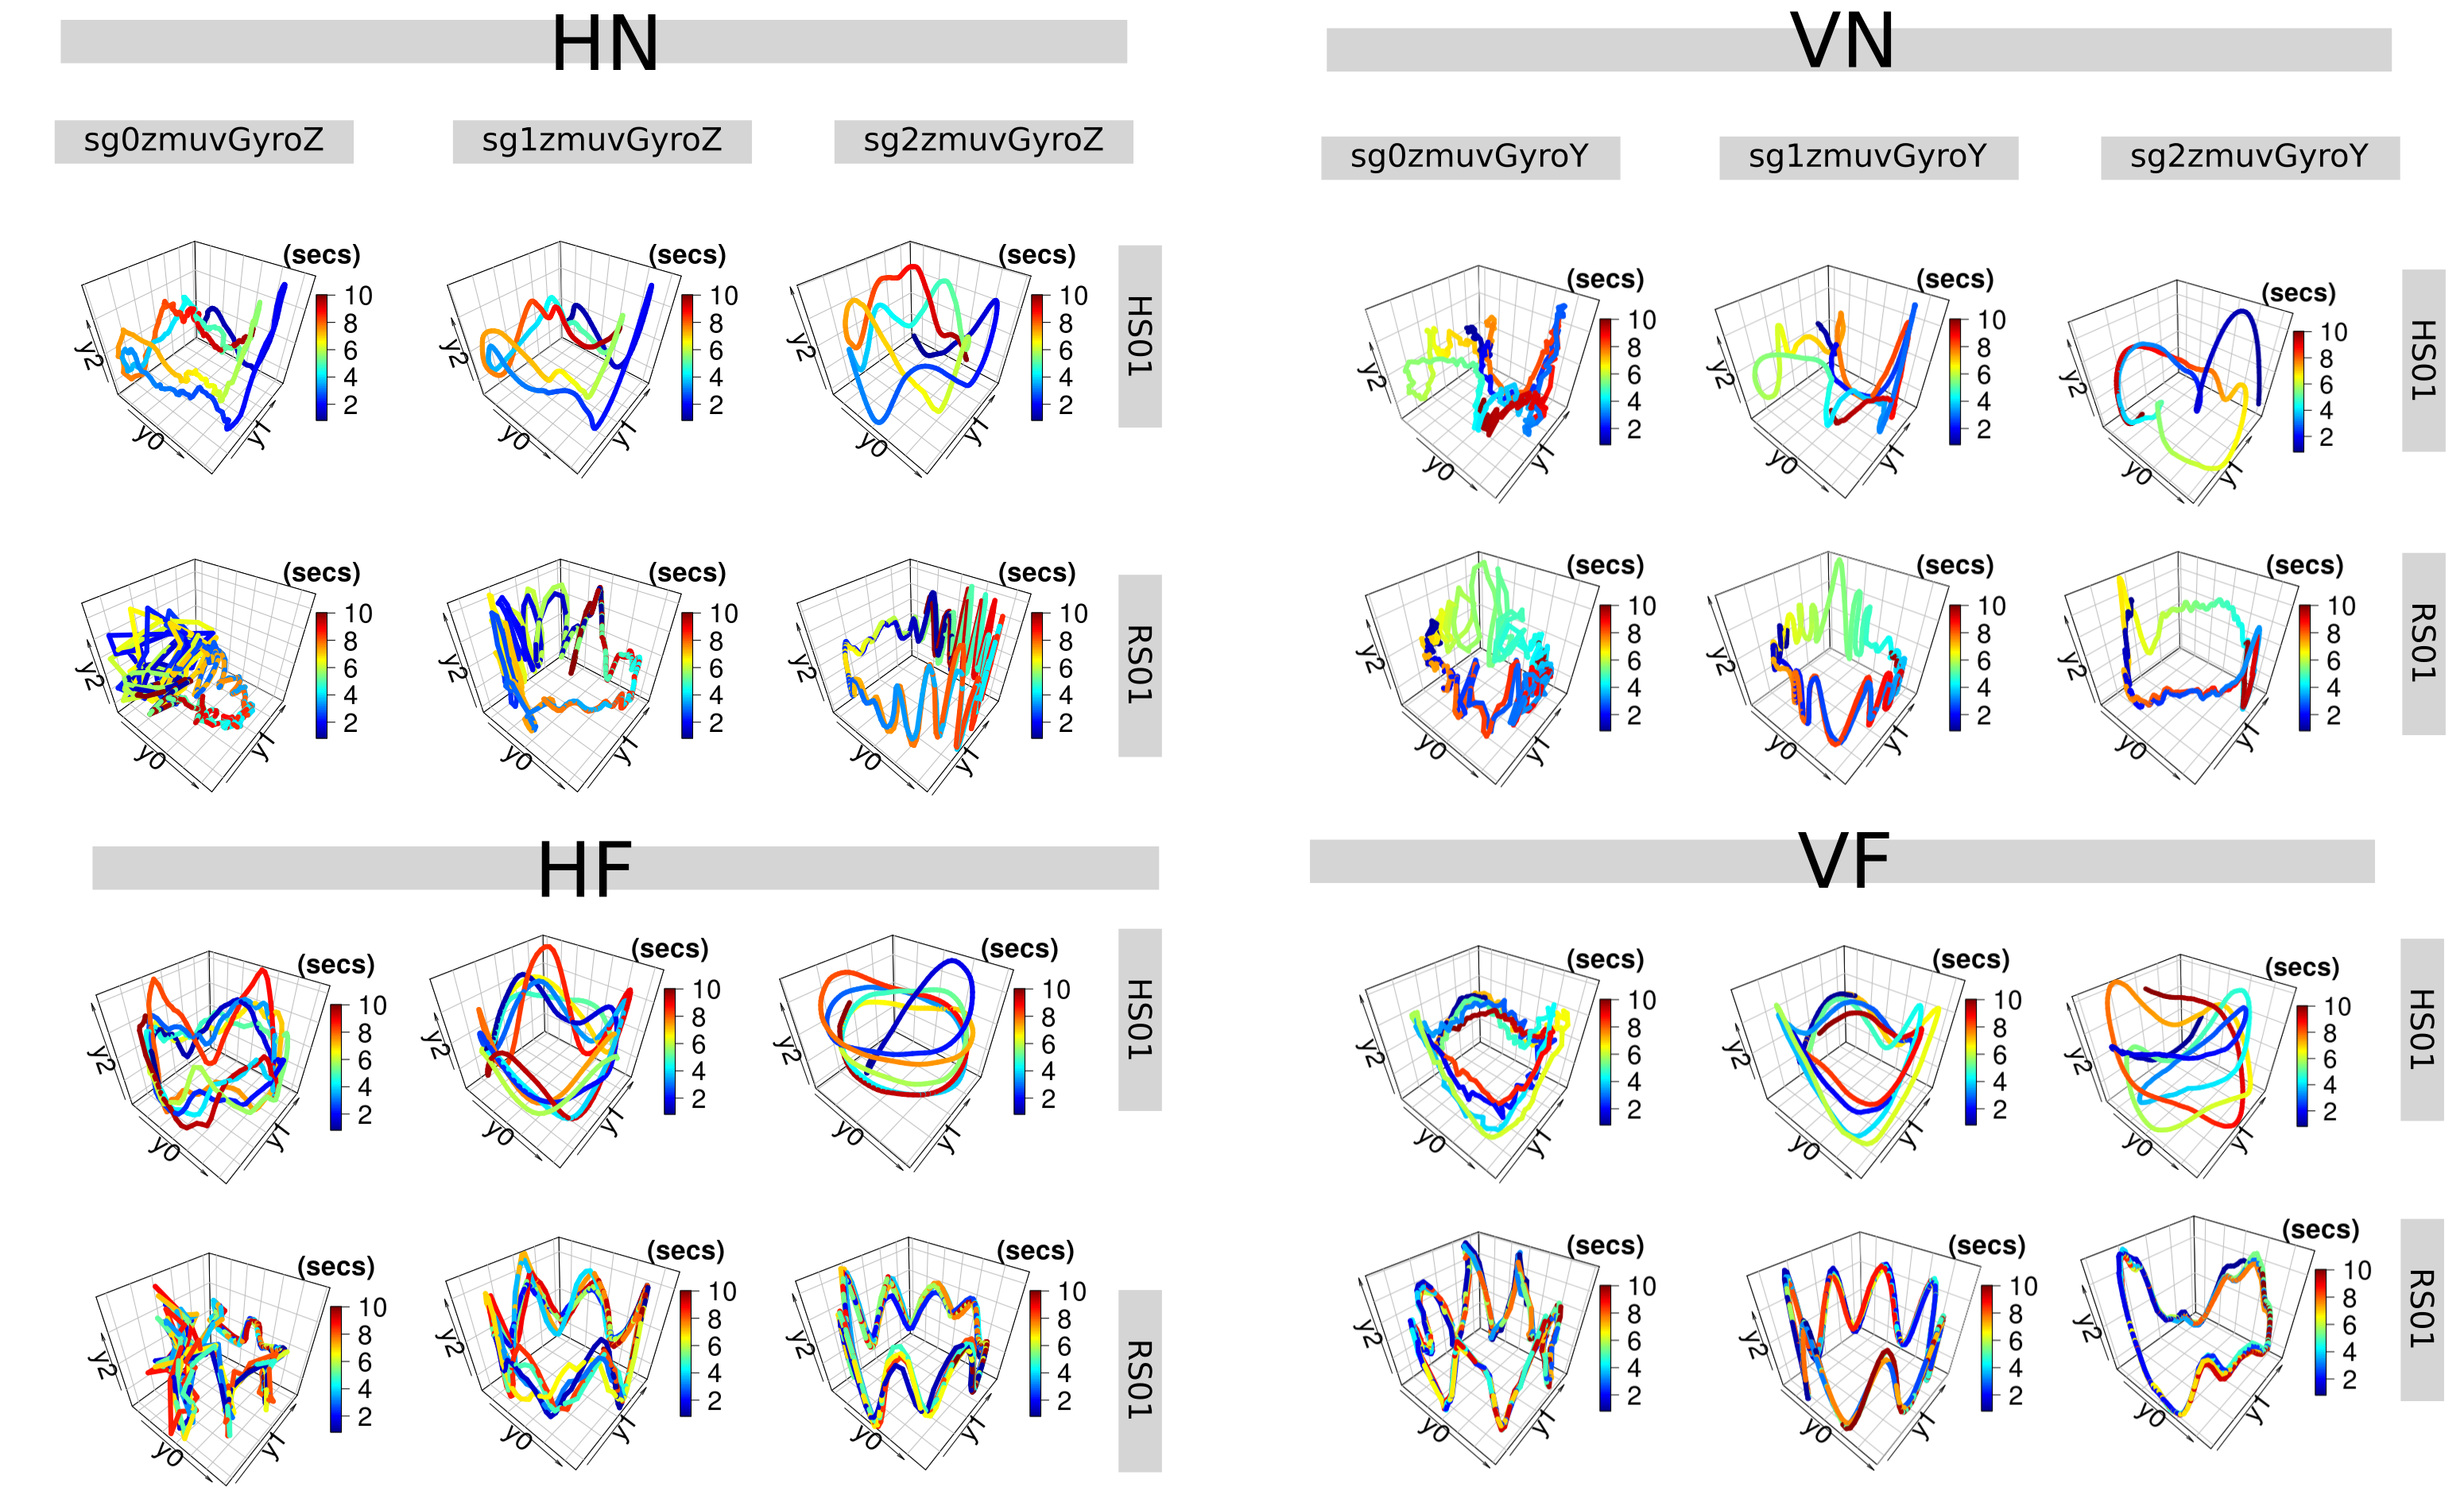
\includegraphics[width=0.8\linewidth]{./figs/results/ch6-rss/versions/drawing-v00}{}
	\caption{RSS for participant 01 computed with ($m=6$, $\tau=8$)
	for different activities, signals and source of time-series data.
	} 
   \end{figure}
\end{frame}
}





%%%%%%%%%%%%%%%%%%%%%%%%%%%%%%%%%%%%%%%%%%%%%%%%%%%%%%%
{
%\paper{Xochicale 2019 in {\bf PhD Thesis}}
\begin{frame}{Recurrence Plots}
    \begin{figure}
        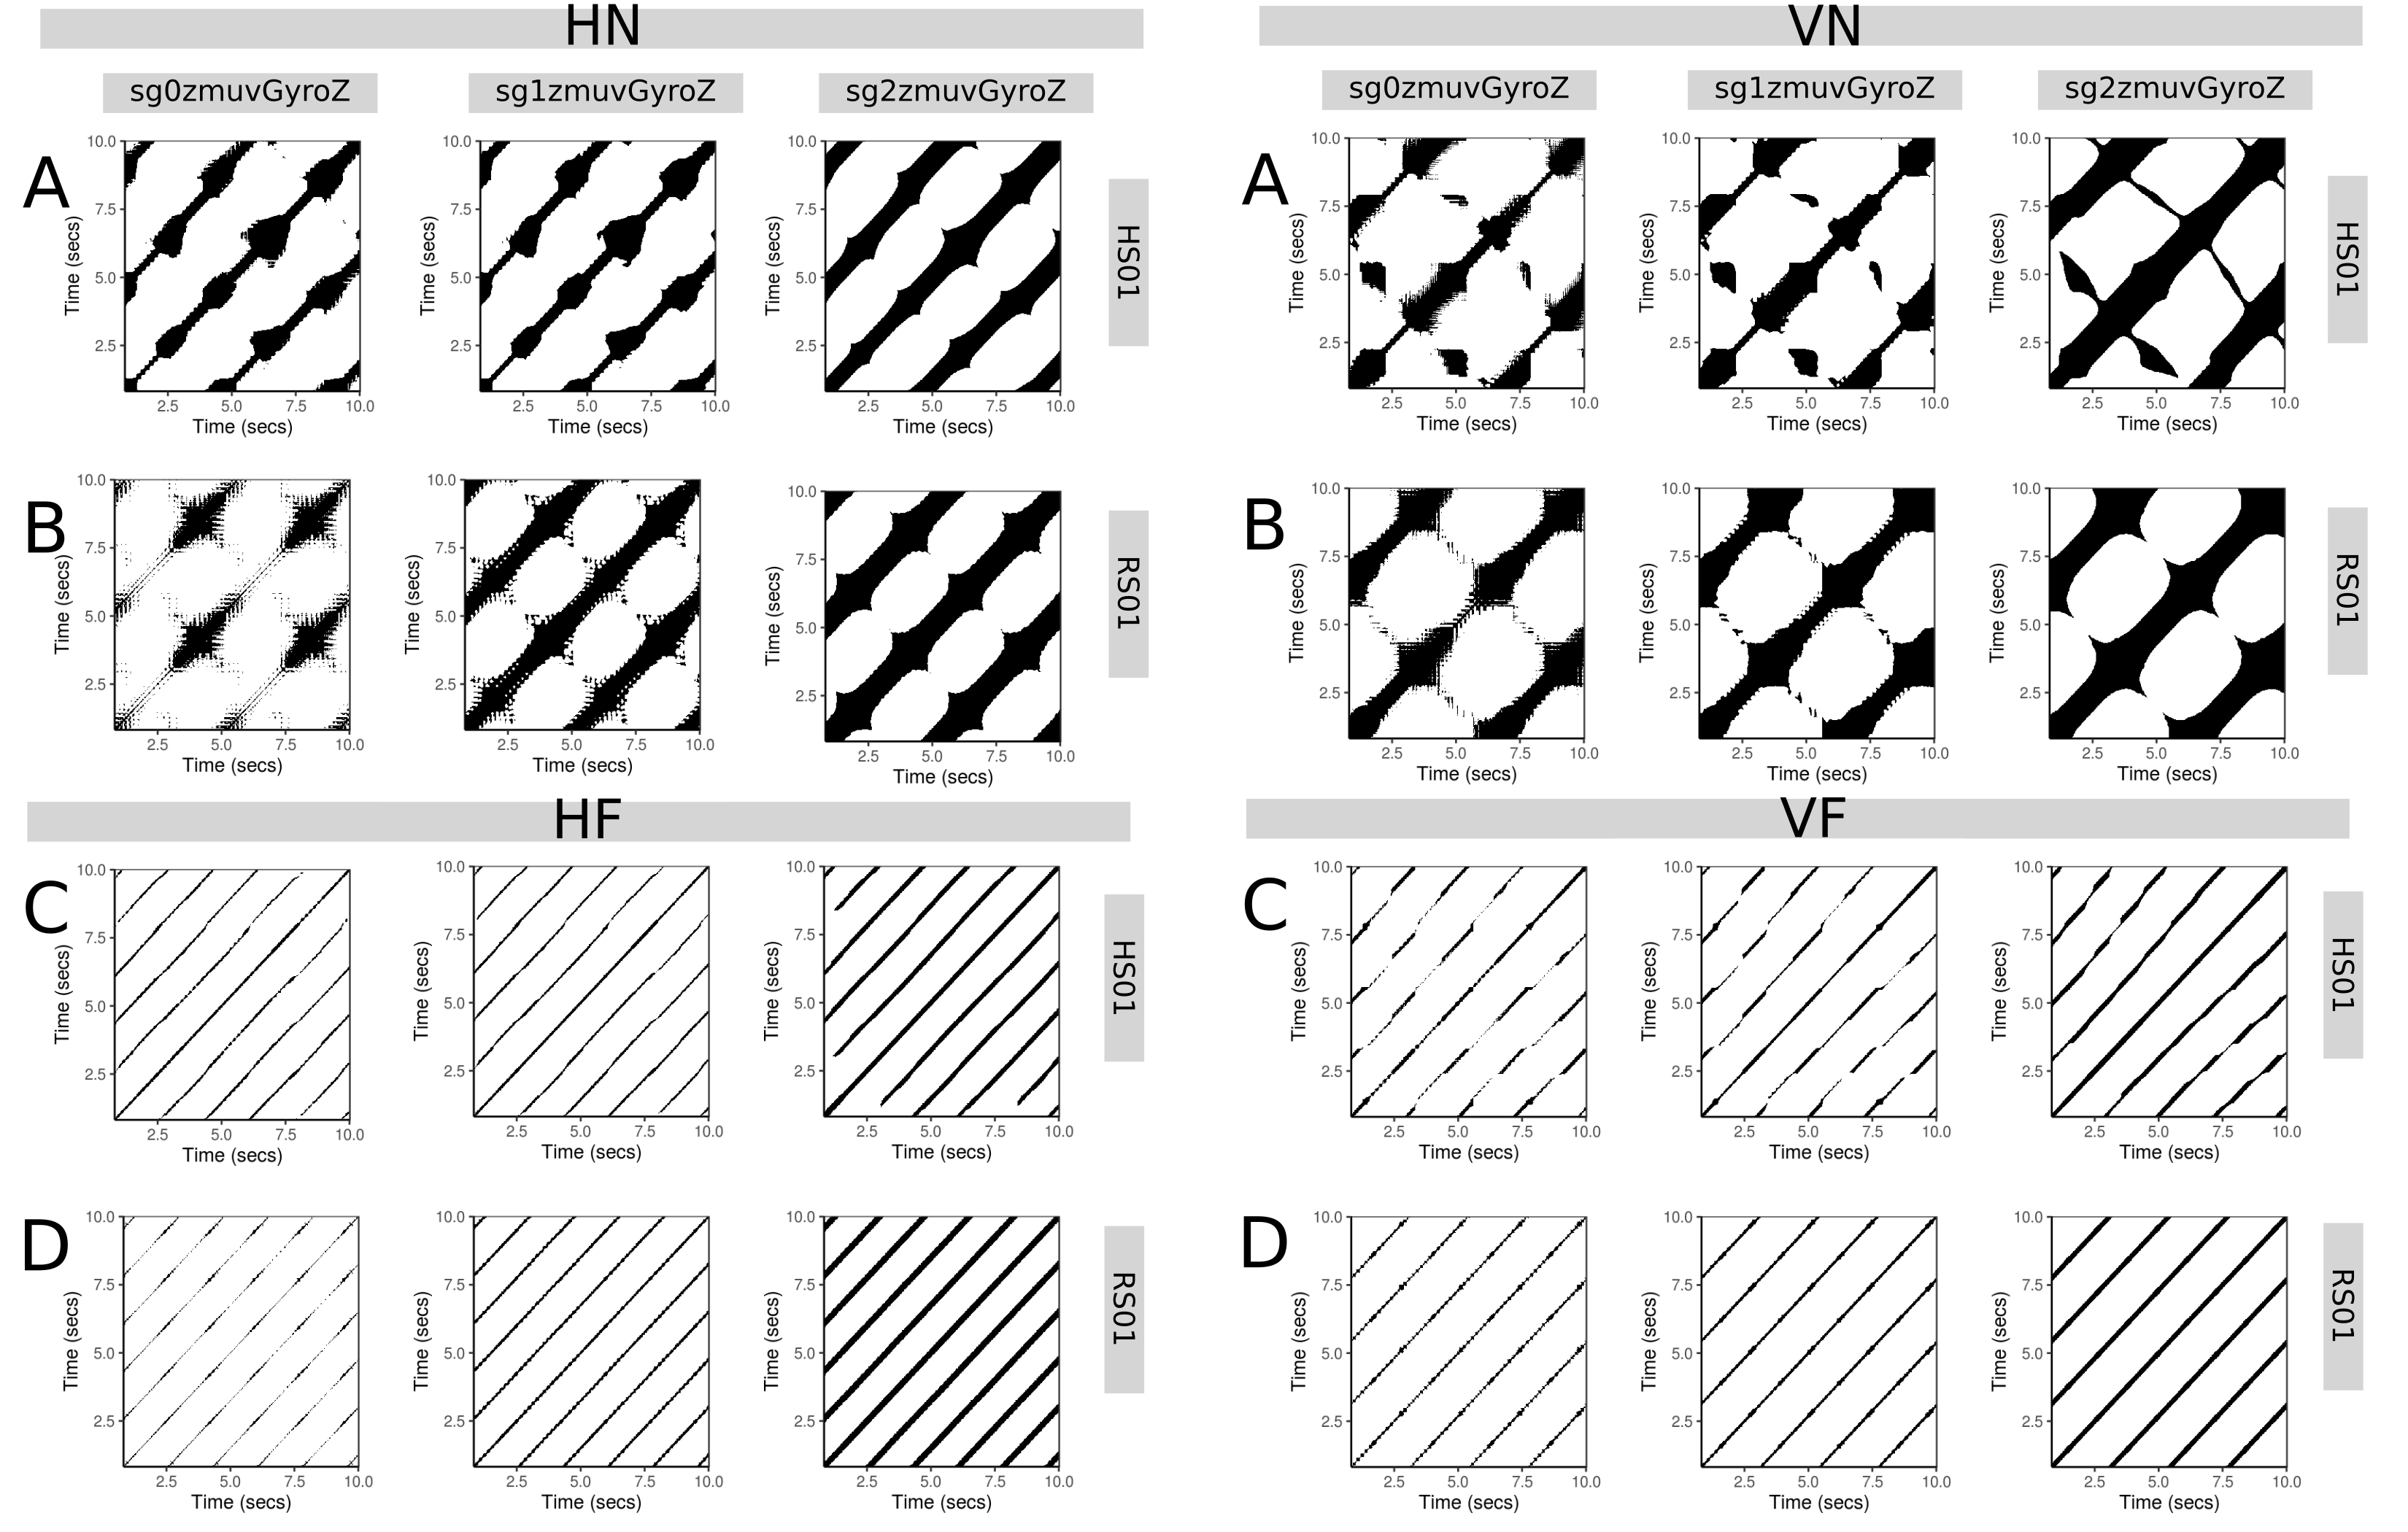
\includegraphics[width=0.8\linewidth]{./figs/results/ch6-rp/versions/drawing-v00}{}
	\caption{RP for participant 01 computed 
	with ($m=6$, $\tau=8$, $\epsilon=1$)
	for different activities, signals and source of time-series data.
	} 
   \end{figure}
	
\end{frame}
}




%%%%%%%%%%%%%%%%%%%%%%%%%%%%%%%%%%%%%%%%%%%%%%%%%%%%%%%
{
\paper{Xochicale 2019 in {\bf PhD Thesis}}

\begin{frame}{Recurrence Quantification Analysis}
    \begin{figure}
        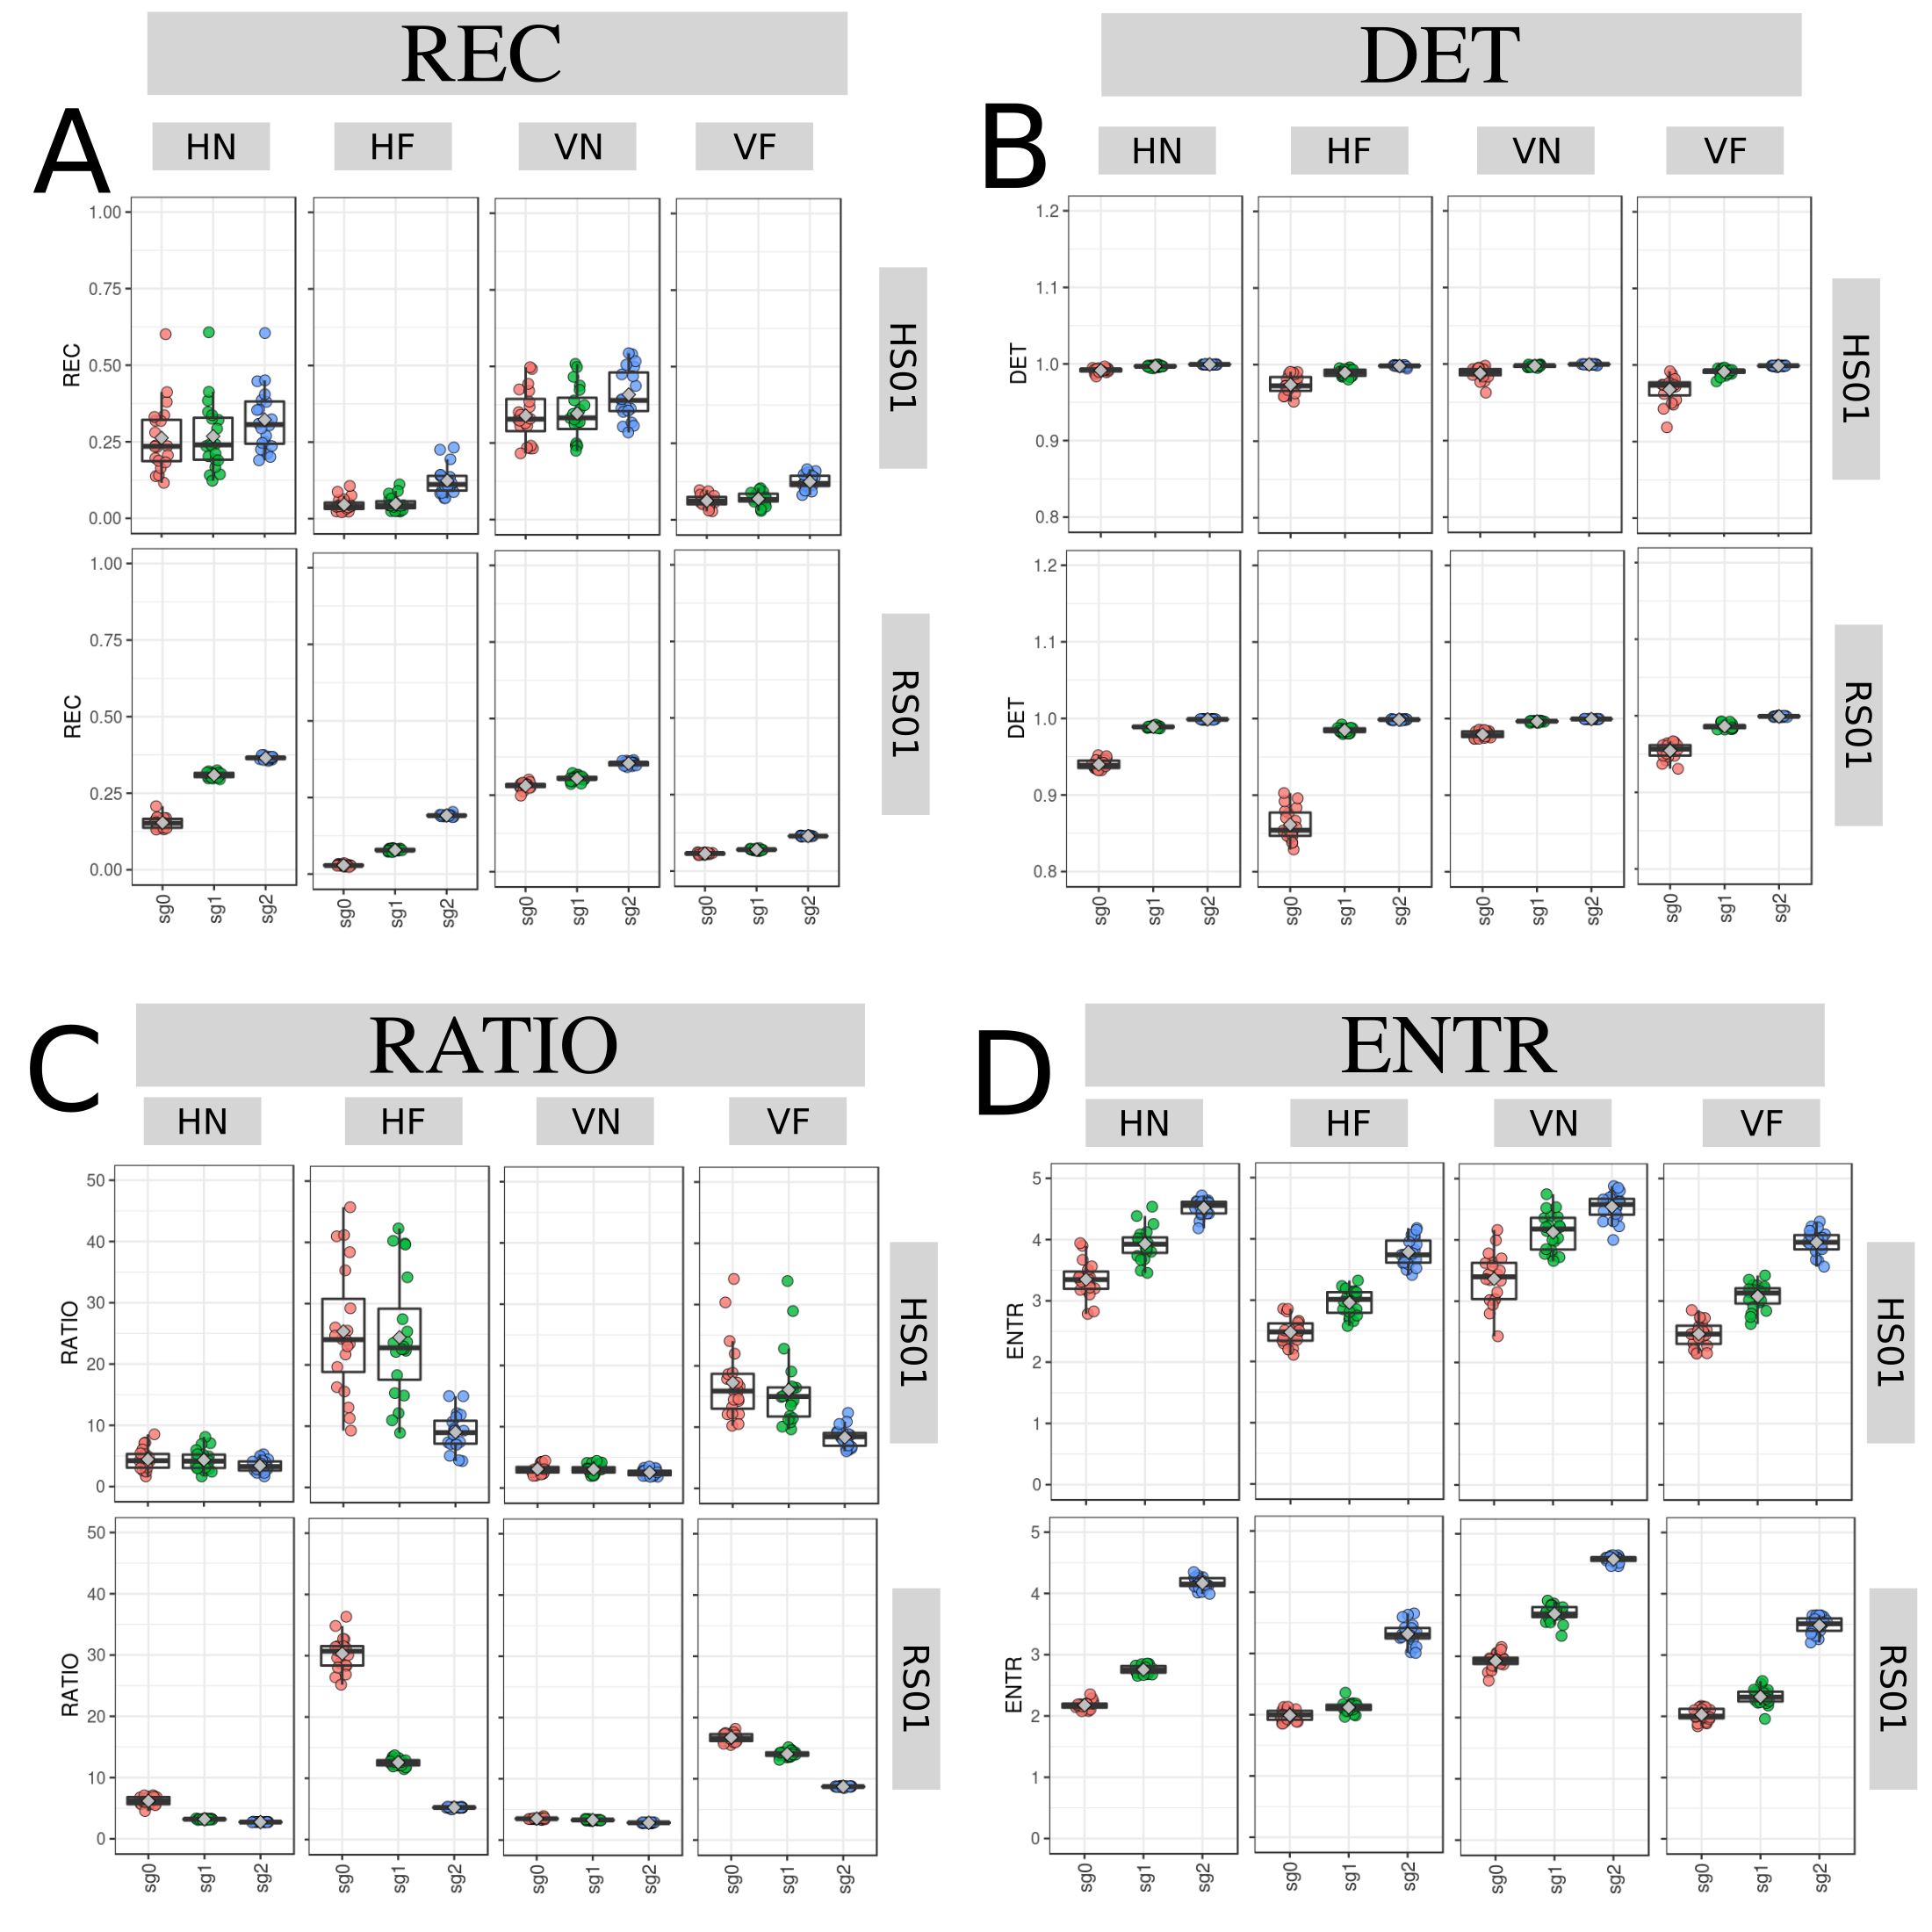
\includegraphics[width=0.45\linewidth]{./figs/results/ch6-rqa/versions/drawing-v00}{}
	\caption{Box values of  RQA computed with 
	($m=7$, $\tau=5$, $\epsilon=1$). 
	These values are for 20 participants.
} 
   \end{figure}
	
\end{frame}
}


%%%%%%%%%%%%%%%%%%%%%%%%%%%%%%%%%%%%%%%%%%%%%%%%%%%%%%%
{
\paper{Xochicale 2019 in {\bf PhD Thesis}}

\begin{frame}{RQA ENTR for $\epsilon$ thresholds
	\& smoothness
}
    \begin{figure}
        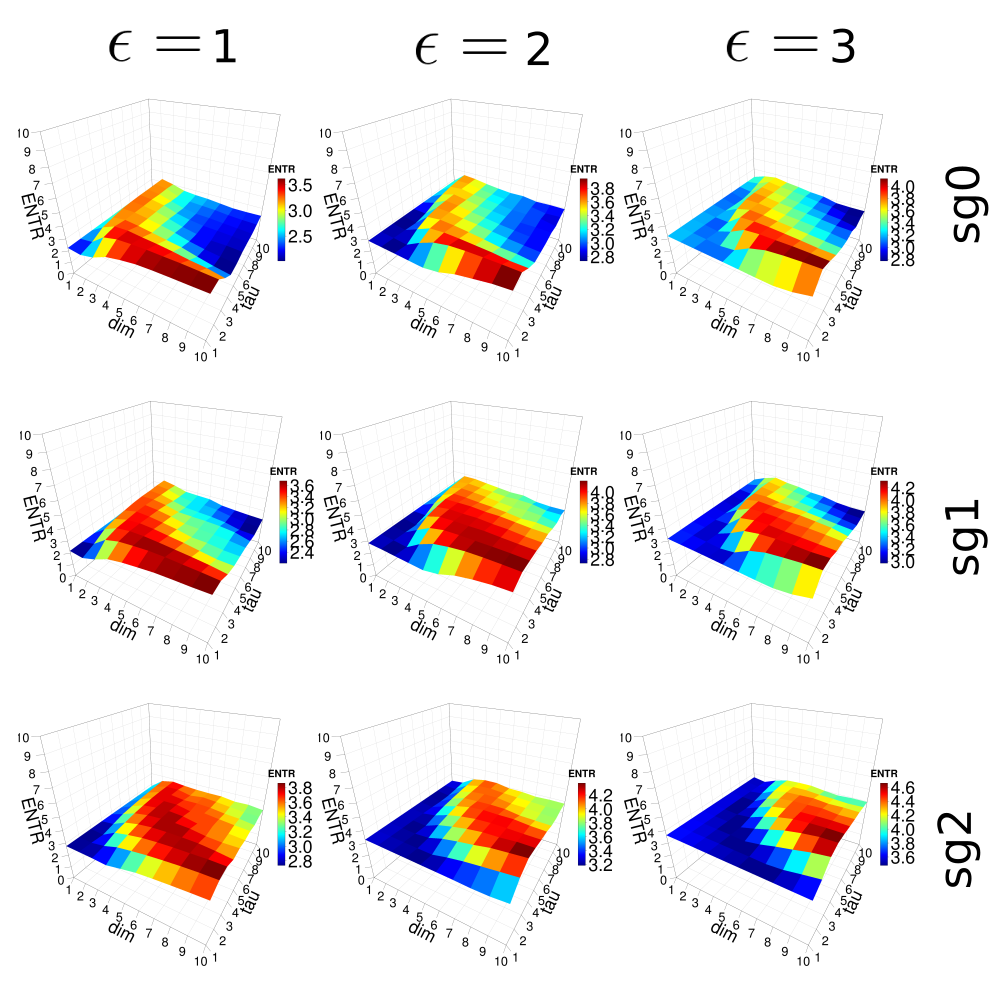
\includegraphics[width=0.45\linewidth]{./figs/results/rqa-epsilons/versions/drawing-v00}{}
	\caption{
	RQA ENTR values are for
	$p03$, sensor $HS01$, of a window size of 10-secs (500 samples).
} 
   \end{figure}
	
\end{frame}
}



%%%%%%%%%%%%%%%%%%%%%%%%%%%%%%%%%%%%%%%%%%%%%%%%%%%%%%%
{
\paper{Xochicale 2019 in {\bf PhD Thesis}}

\begin{frame}{RQA ENTR for sensors and activities
}
    \begin{figure}
        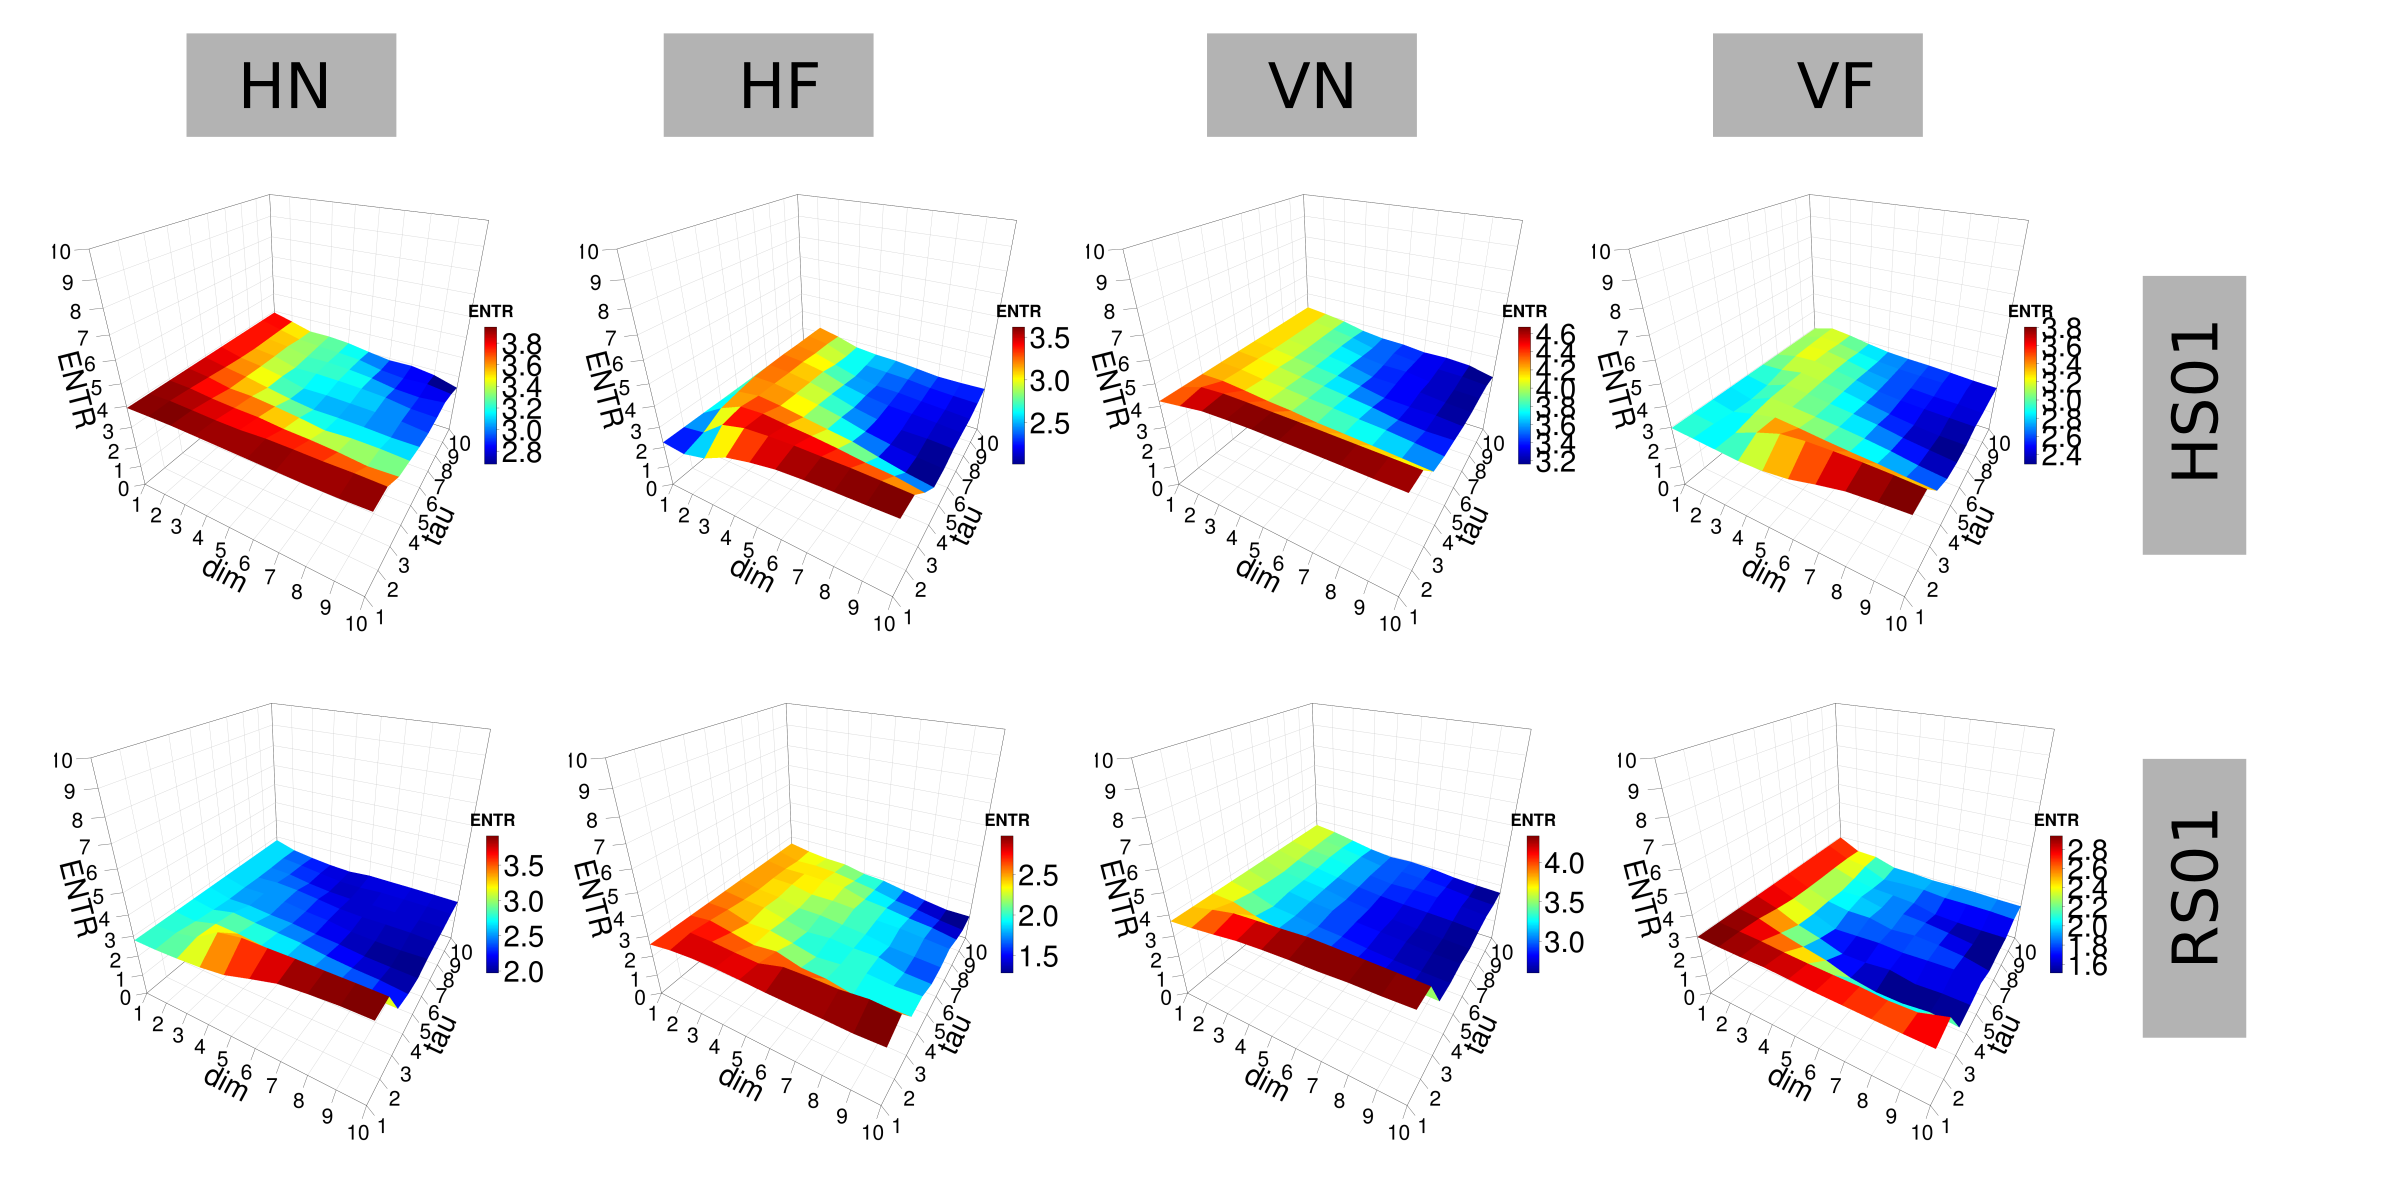
\includegraphics[width=0.75\linewidth]{./figs/results/rqa-epsilons-sensors-activities/versions/drawing-v00}{}
	\caption{
	RQA ENTR values are for
	$p03$, $sg0$ and window size of 10-secs (500 samples).
} 
   \end{figure}
	
\end{frame}
}







\subsection{}
%%%%%%%%%%%%%%%%%%%%%%%%%%%%%%%%%%%%%%%%%%%%%%%%%%%%%%%
{
\paper{Xochicale 2019 in {\bf PhD Thesis}}

\begin{frame}{Window size lengths
}
   \begin{figure}
        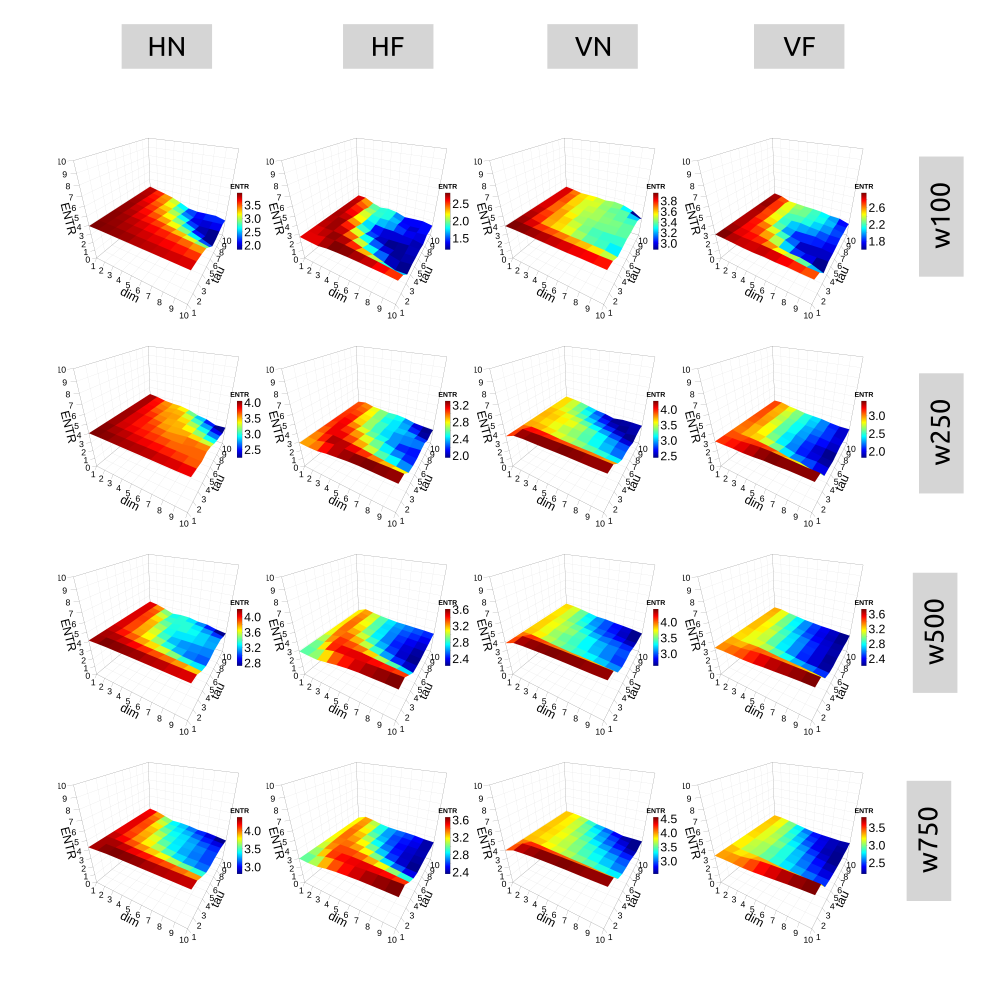
\includegraphics[width=0.55\linewidth]{./figs/results/3d-rqa-epsilons-windows/versions/drawing-v00}{}
	\caption{Window length size effect on 3D surface plots of RQA.} 
   \end{figure}
	
\end{frame}
}









\subsection{}
%%%%%%%%%%%%%%%%%%%%%%%%%%%%%%%%%%%%%%%%%%%%%%%%%%%%%%%
{
\paper{Xochicale 2019 in {\bf PhD Thesis}}

\begin{frame}{Participants
}
    \begin{figure}
        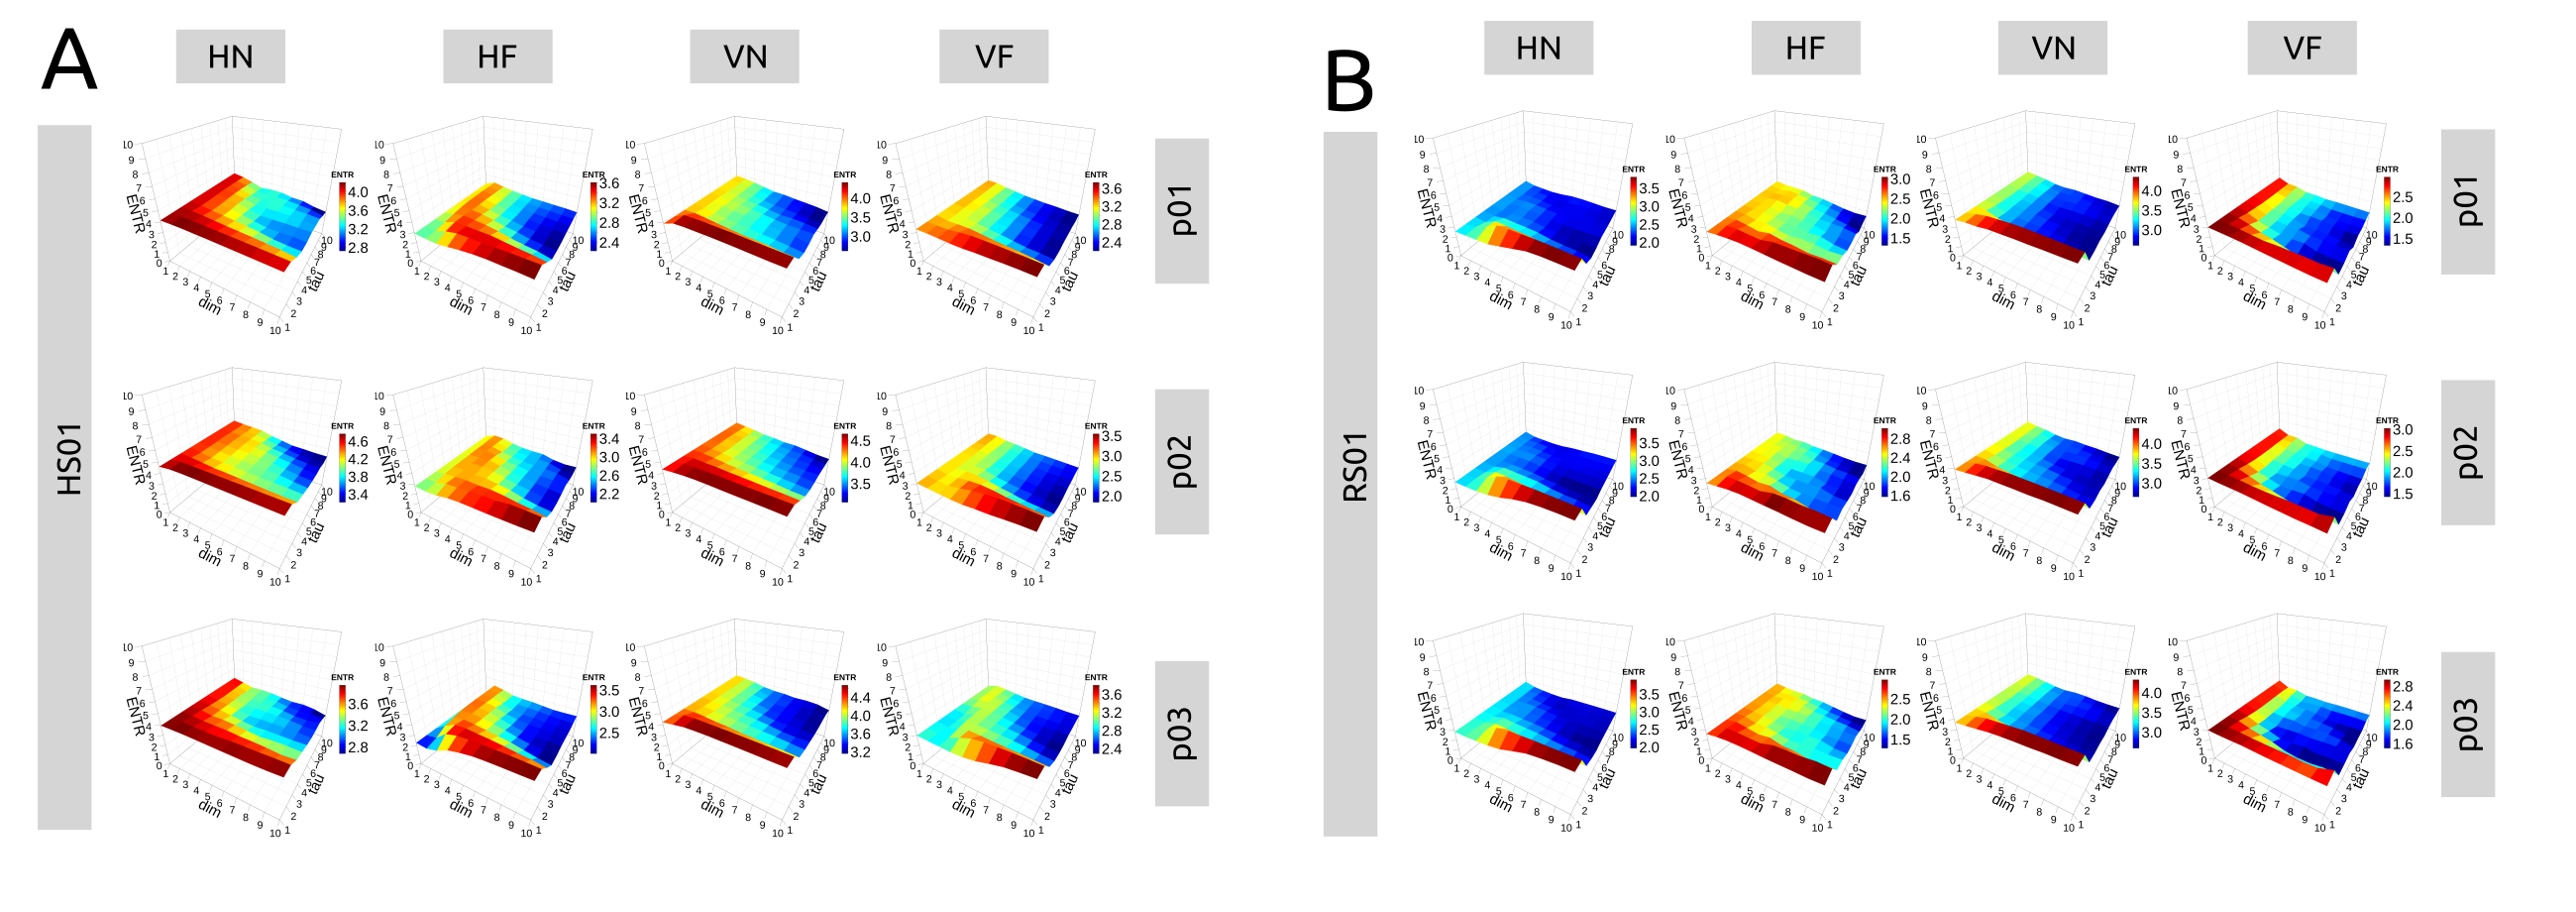
\includegraphics[width=1.0\linewidth]{./figs/results/3d-rqa-epsilons-participants/versions/drawing-v00}{}
	\caption{Participants differences of 3D surface plots of RQA.} 
   \end{figure}
	
\end{frame}
}


%%%%%%%%%%%%%%%%%%%%%%%%%%%%%%%%%%%%%%%%%%%%%%%%%%%%%%%%%
%{
%\paper{Xochicale 2019 in {\bf PhD Thesis}}
%
%\begin{frame}{3D surfaces plots of RQA
%	{\bf (in preparation)}
%}
%    \begin{figure}
%        \centering
%        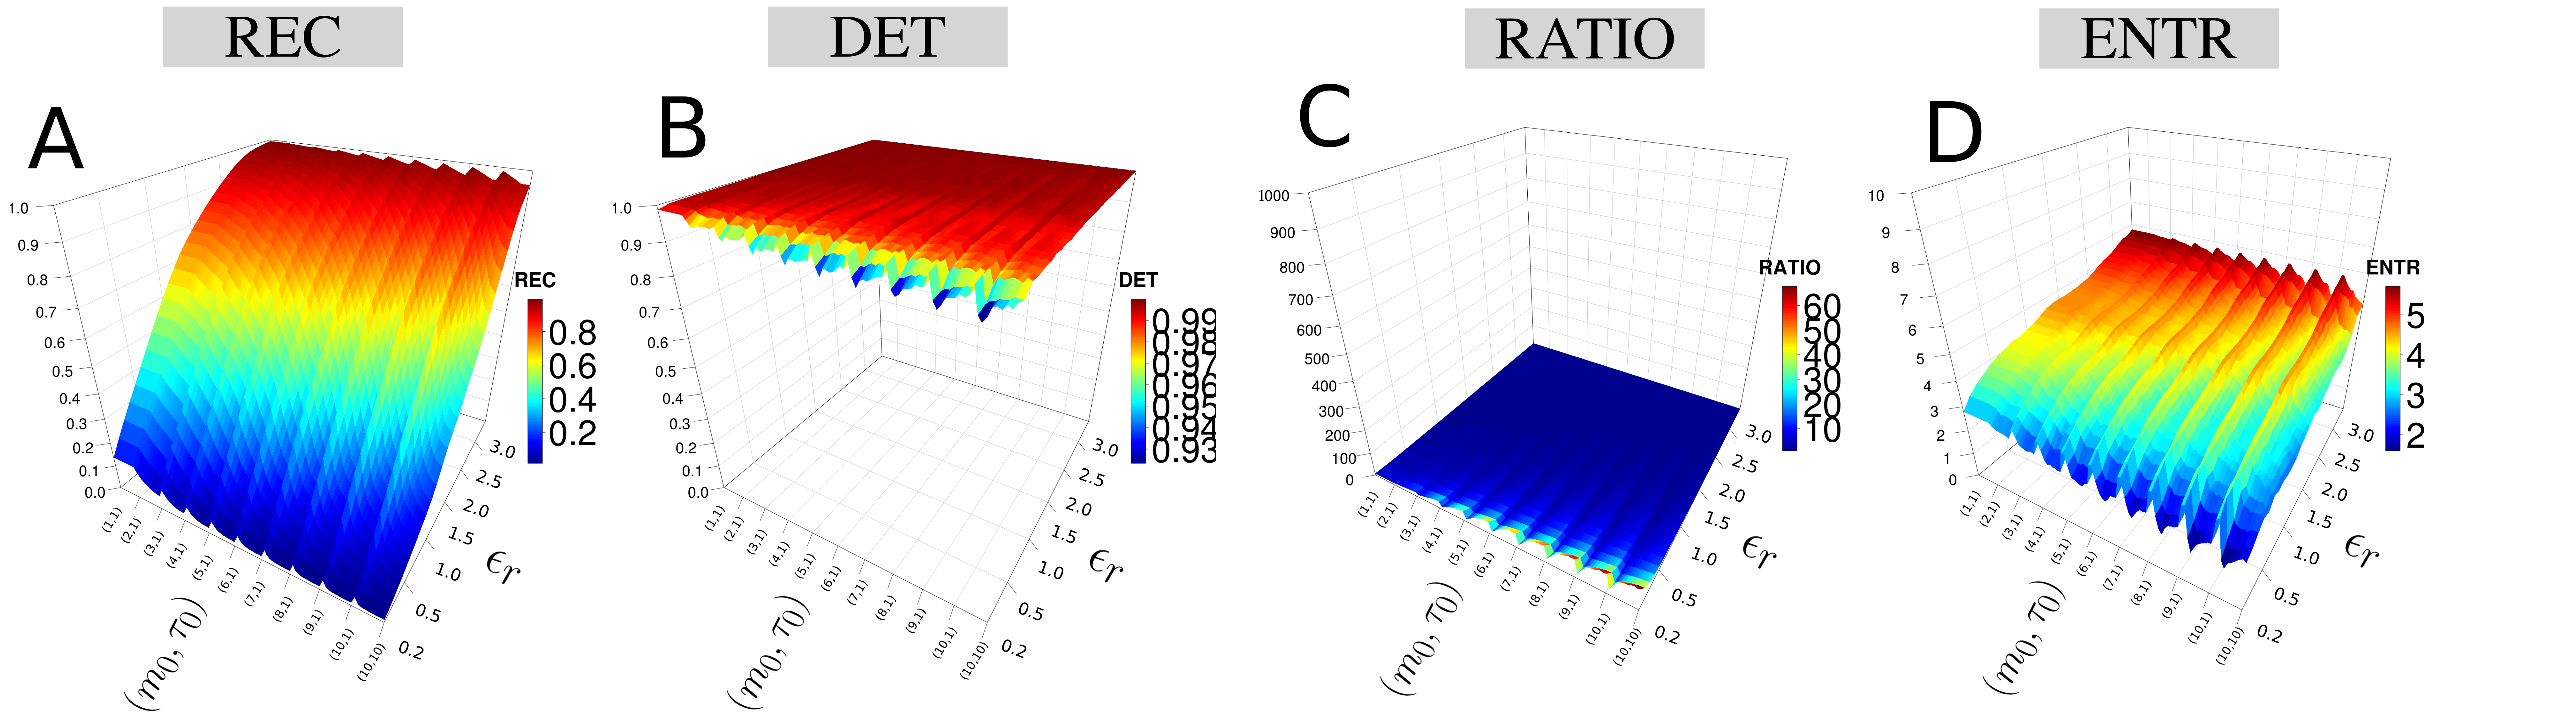
\includegraphics[width=0.75\linewidth]{./figs/results/3d-rqa/versions/drawing-v00}{}
%	\small
%	\caption{
%		3D RQA surfaces 
%	with increasing pair of embedding parameters 
%	($0 \le m \le 10$, $0 \le \tau \le 10$) 
%	and recurrence thresholds ($ 0.2 \le \epsilon \le 3 $).
%	} 
%   \end{figure}
%	
%\end{frame}
%}
%

%%%%%%%%%%%%%%%%%%%%%%%%%%%%%%%%%%%%%%%%%%%%
\subsection{Conclusions}



{
{
\paper{Zia et al., 2017 in {\bf Computer Assisted Radiology and Surgery};
Mori 2012 in {\bf Development and Learning and Epigenetic Robotics};
Mitsukura et al., 2017 in {\bf Electroencephalography}; 
Marwan et al. 2019 in {\bf http://recurrence-plot.tk/}
}
\begin{frame}{Applications of Nonlinear Dynamics}
    \vspace{-02mm}
    \begin{figure}
        \centering
        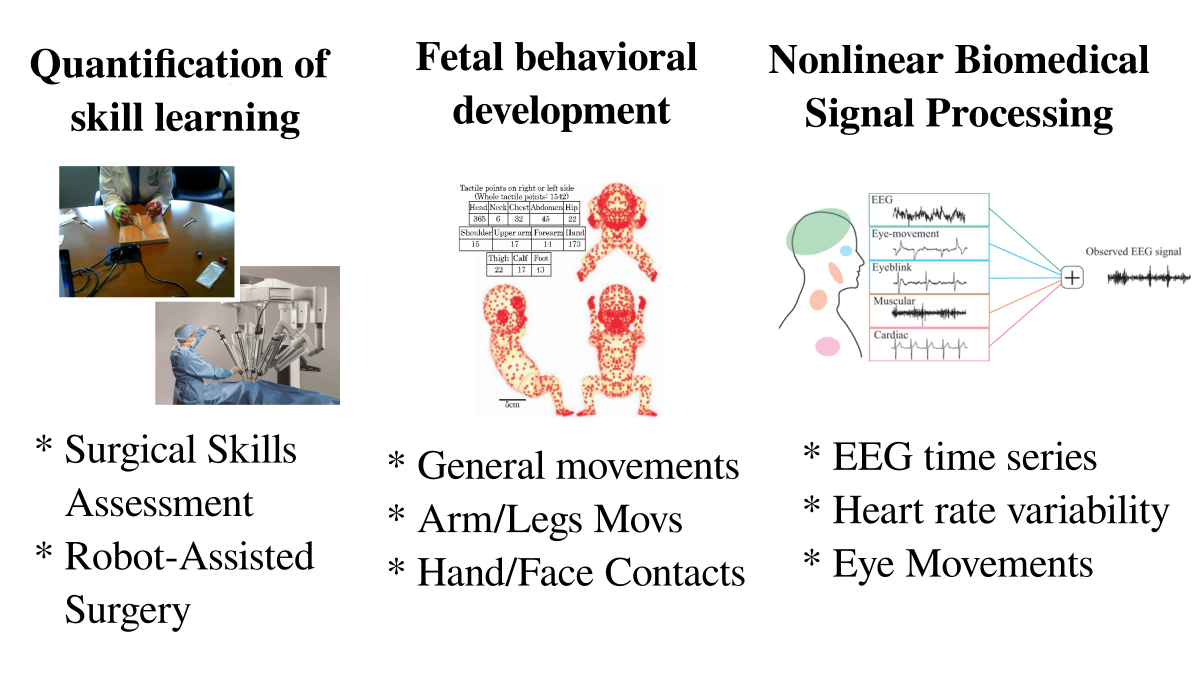
\includegraphics[width=0.9\linewidth]{./figs/applications/versions/drawing-v00.png}
	%\caption{} 
   \end{figure}
	
\end{frame}
}


%%%%%%%%%%%%%%%%%%%%%%%%%%%%%%%%%%%%%%%%%%%%%%%%%%%%%%%%
{
%\paper{Xochicale 2019 in {\bf PhD thesis}}

\begin{frame}{Conclusions and future work}

\textbf{Take away messages}
\begin{itemize}
\item Nonlinear analysis tools can quantify different
data time-series. 
\item Shannon entropy with 3D plot surfaces of RQA appear to be robust for real-word data (i.e. different time series
structures, window length size and levels of smoothness).
\item Therefore, Shannon entropy would be a potential good tool to quantify complexity of movement.
%\item Smoothing raw time series can create well defined trajectories
%or patterns in RSS or RP, however such increase of smoothness 
%can also create more complex (i.e. not well defined) trajectories
%or patterns in nonlinear analysis. 

\end{itemize}

\textbf{Investigate}
\begin{itemize}
	\item other methodologies for state space reconstruction,
	\item the robustness of Entropy measurements with RQA, and 
	\item variability in perception of velocity.
\end{itemize}




\end{frame}
}






%%%%%%%%%%%%%%%%%%%%%%%%%%%%%%%%%%%%%%%%%%%%
\section{Extras}


%%%%%%%%%%%%%%%%%%%%%%%%%%%%%%%%%%%%%%%%%%%%
\subsection{Ultrasound Needle Tracking}

{
\paper{
\textbf{Xia et. al., 2017} in Scientific Reports DOI:10.1038/s41598-017-03886-4; 
\textbf{Xia et. al., 2016} in MICCAI DOI:10.1007/978-3-319-46720-741
}

\begin{frame}{Ultrasound needle tracking}

\begin{columns}

\begin{column}{.6\linewidth}
	\begin{figure}
        \centering
        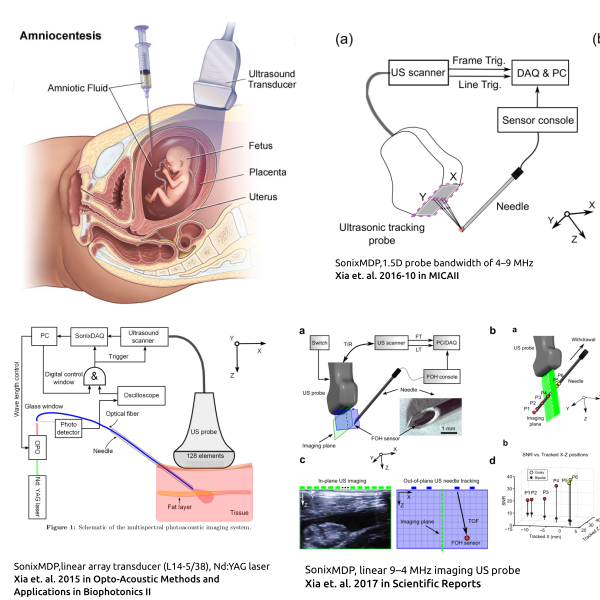
\includegraphics[scale=0.4]{./figs/unt/versions/drawing-v00}
        %\caption{}
      \end{figure}
\end{column}

\begin{column}{.4\linewidth}
	\textbf{Challenges}
        \begin{itemize}
         %\item To see the needle, the ultrasound probe needs to be moved.
	 \item In-plane and out-plane needle tracking
	 \item Needle manipulation is impacted by the experience of the clinitians
	 \item The anatomical view changes.
        \end{itemize}	
\end{column}



\end{columns}

\end{frame}
}



%%%%%%%%%%%%%%%%%%%%%%%%%%%%%%%%%%%%%%%%%%%%
\subsection{free-corTeX: a free CI framework for open scientific communication}
{
\paper{\textbf{Xochicale 2020} in Conf. of Reproducibility, Replicability and Trust in Science \faGithub github.com/mxochicale/rrts2020}

\begin{frame}{
free-corTeX: a free CI framework for open scientific communication
}

      \begin{figure}
        \centering
        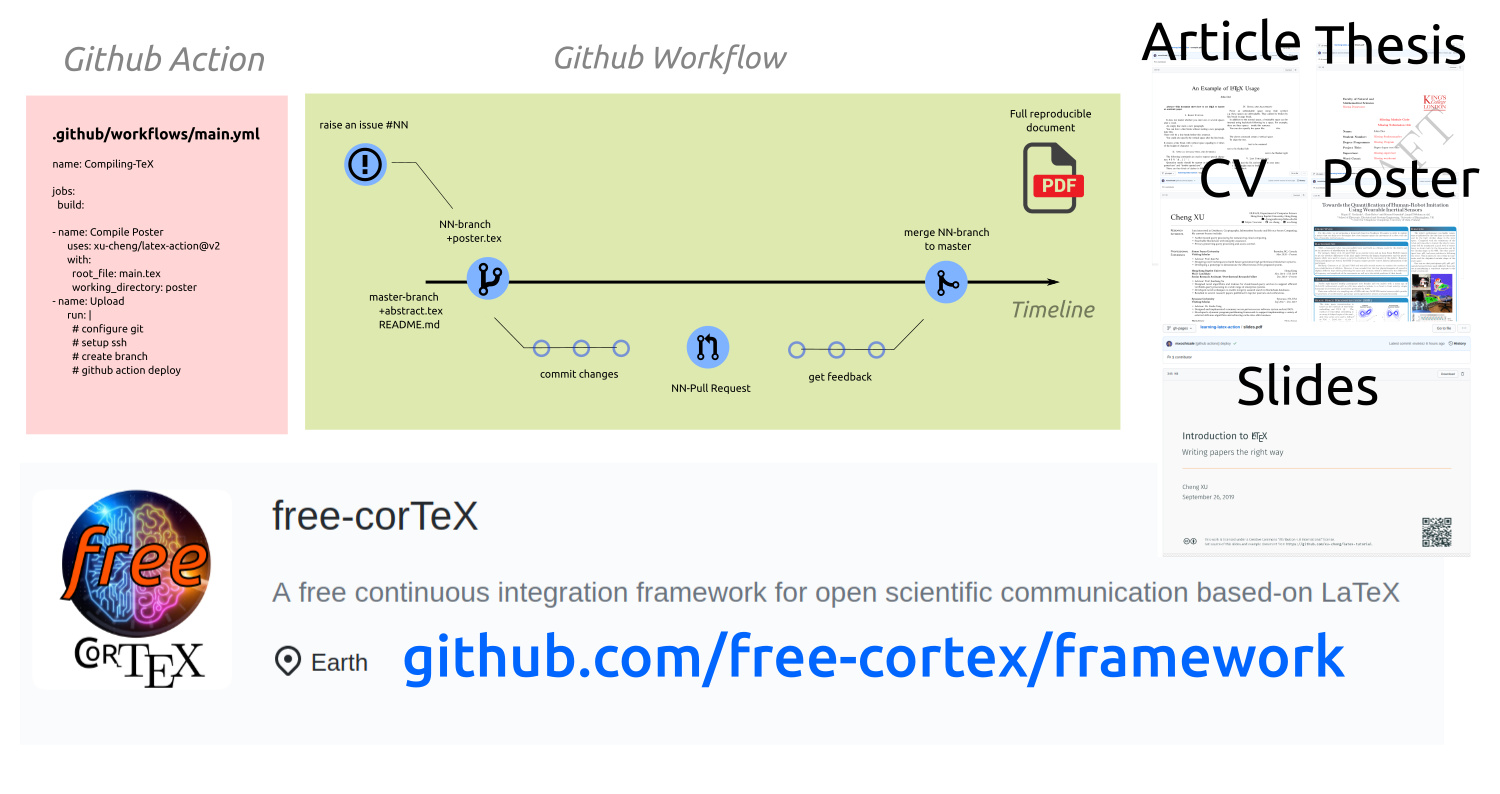
\includegraphics[width=0.95\textwidth]{./figs/free-cortex/versions/drawing-v01.png}
        %\caption{}
      \end{figure}

\end{frame}
}


%%%%%%%%%%%%%%%%%%%%%%%%%%%%%%%%%%%%%%%%%%%%
\subsection{air4children}

%%%%%%%%%%%%%%%%%%%%%%%%%%%%%%%%%%%%%%%%%%%%%%%%%%%%%%%%
{
\paper{
{
\faGithub https://github.com/air4children
}
}
\begin{frame}{AIR4Children: Artificial Intelligence and Robotics for Children}

\begin{columns}

\begin{column}{.6\linewidth}
      \begin{figure}
        \centering
        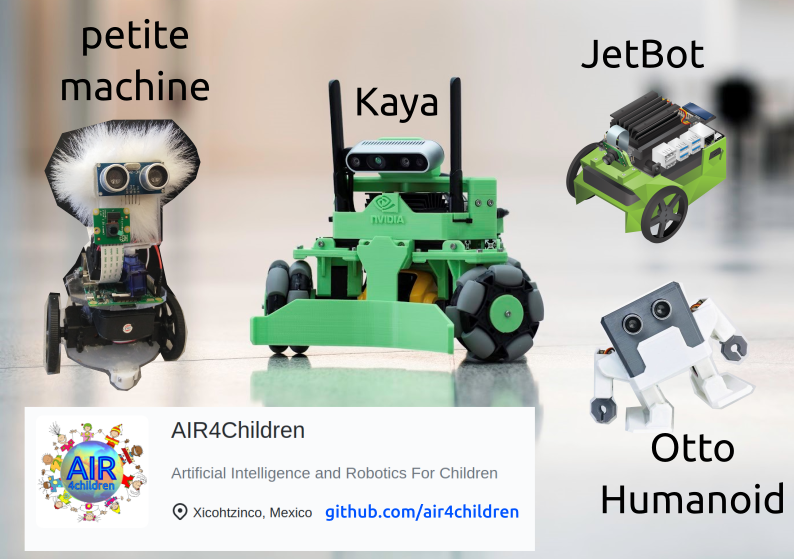
\includegraphics[width=1.0\textwidth]{./figs/air4children/versions/drawing-v00.png}
        %\caption{}
      \end{figure}
\end{column}

\begin{column}{.4\linewidth}
	Free teaching of AI and Robotics for Children with
	\textbf{Open-Sourced Robots that are:}
        \begin{itemize}
         %\item To see the needle, the ultrasound probe needs to be moved.
	 \item Affordable,
	 \item Educational, and
	 \item Fun.
        \end{itemize}	
\end{column}

\end{columns}

\end{frame}
}



%\subsection{References}
%%%%%%%%%%%%%%%%%%%%%%%%%%%%%%%%%%%%%%%%%%%%%%%%%%%%%%%%
\begin{frame}{References}
    \begin{thebibliography}{10}

\beamertemplatearticlebibitems

	\bibitem{xochicale2020}
	Xochicale Miguel
	\newblock 
	Nonlinear methods to quantify Movement Variability 
	in Human-Humanoid Interaction Activities
	\newblock Submission in progress to Scientific Reports  
      	\newblock \url{https://arxiv.org/abs/1810.09249}

    \end{thebibliography}
\end{frame}


\title{Thanks!!! Questions?}
\subtitle{
	Nonlinear analysis to quantify human movement variability from time-series data \\
	\url{https://github.com/mxochicale/seminario-cicese-27112020}
}
\date{}
\maketitle



\end{document}
